\documentclass[10pt, a4paper]{scrartcl}
% Packages
\usepackage[margin=1.25in]{geometry}
\usepackage{index}
\makeindex
\usepackage[utf8]{inputenc}
\usepackage[T1]{fontenc}
\usepackage{tcolorbox}
\tcbuselibrary{theorems}
\tcbuselibrary{skins}
\tcbuselibrary{breakable}
\usepackage{varwidth}
\usepackage{amsmath, amssymb}
\usepackage{esint}
\usepackage{titlesec}
\usepackage{xcolor}
\usepackage{titling}
\usepackage[linktocpage]{hyperref}
\usepackage{pgfplots}
\usepackage{caption}
\usepackage{amsthm}
\usepackage{import}
\usepackage{cancel}
\usepackage{caption}
\usepackage{nicematrix}
\usepackage{mathtools}
\usepackage{mathrsfs}
\usepackage{enumerate}
\usepackage{graphicx}
\usepackage{tikz}
\usepackage[italian]{babel}
\usepackage{setspace}
%\usepackage{cmupint}
\usepackage[perpage]{footmisc} % To reset footnote numbering each page
\setstretch{1.2}

% Titles 
\title{Note di Analisi 2}
\author{Manuel Deodato}
\date{}


% svolgimento
\newenvironment{svolgimento}{\renewcommand\qedsymbol{$\blacksquare$}\begin{proof}[Svolgimento]}{\end{proof}}


%%%%% tcolorbox setup

% Teorema e proposizione
\newtcbtheorem[number within=section]{teorema}{Teorema}
{breakable, top=0.2mm, bottom=0.2mm, boxrule=0mm,arc =.5 mm, colframe=blue!10, coltitle=black, fonttitle=\bfseries, colback=blue!5!white, theorem style=plain apart}{th}

\newtcbtheorem[number within=section]{prop}{Proposizione}
{breakable, top=0.2mm, bottom=0.2mm, boxrule=0mm,arc =.5 mm, colframe=blue!10, coltitle=black, fonttitle=\bfseries, colback=blue!5!white, theorem style=plain apart}{prop}





% Definizione
\definecolor{greendef}{HTML}{b8d8be}

\newtcbtheorem[number within=section]{definizione}{Definizione}
{breakable, top=0.2mm, bottom=0.2mm, boxrule=0mm, arc=.5mm, colframe=greendef, coltitle=black, fonttitle=\bfseries, theorem style = plain apart, colback=greendef!50!white}{def}


% Esempio
\theoremstyle{definition}
\newtheorem{esempio}{Esempio}

%\definecolor{empurple}{HTML}{6e5e89}

%\newtcbtheorem{esempio}{Esempio}{left=0mm,arc=0mm, colframe=empurple!10!white, coltitle=black, fonttitle=\bfseries, theorem style = plain, colback=empurple!20!white, colframe=empurple!90!white, boxrule=1pt, sharp corners, top=.2mm,bottom=.2mm}{es}

\tcolorboxenvironment{esempio}{blanker,breakable,left=5mm,before skip=10pt,after skip=10pt, borderline west={1mm}{0pt}{greendef}}

\numberwithin{esempio}{section}


% Lemma e Corollario
\definecolor{lemcor}{HTML}{a78d8a}

\newtcbtheorem[number within=section]{lemma}{Lemma}{breakable, top=0.2mm, bottom=0.2mm, boxrule=0mm,left=0mm,arc=.5mm, colframe=lemcor!10!white, coltitle=black, fonttitle=\bfseries, theorem style = plain apart, colframe=lemcor!50!white,colback=lemcor!20!white}{lem}
\newtcbtheorem[number within=section]{corollario}{Corollario}{breakable, top=0.2mm, bottom=0.2mm, boxrule=0mm,left=0mm,arc=.5mm, colframe=lemcor!10!white, coltitle=black, fonttitle=\bfseries, theorem style = plain apart, colframe=lemcor!50!white,colback=lemcor!20!white}{cor}



% Osservazione
\theoremstyle{definition}
\newtheorem{obs}{Osservazione}

\definecolor{coloros}{HTML}{6e5e89}

\tcolorboxenvironment{obs}{blanker,breakable,left=5mm,before skip=10pt,after skip=10pt, borderline west={1mm}{0pt}{coloros}}

\numberwithin{obs}{section}

% Nota
\newtheorem{nota}{Nota}

\definecolor{ncol}{HTML}{f9ebbe}

\tcolorboxenvironment{nota}{blanker,breakable,left=5mm,before skip=10pt,after skip=10pt, borderline west={1mm}{0pt}{ncol}}

\numberwithin{nota}{section}



%%%%%%%%%% Medie con integrali multipli
\def\Yint#1{\mathchoice
    {\YYint\displaystyle\textstyle{#1}}%
    {\YYint\textstyle\scriptstyle{#1}}%
    {\YYint\scriptstyle\scriptscriptstyle{#1}}%
    {\YYint\scriptscriptstyle\scriptscriptstyle{#1}}%
      \!\iint}
\def\YYint#1#2#3{{\setbox0=\hbox{$#1{#2#3}{\iint}$}
    \vcenter{\hbox{$#2#3$}}\kern-.51\wd0}}
\def\longdash{{-}\mkern-3.5mu{-}} 
   % consider using "\mkern-7.5mu" if esint package is loaded
\def\tiltlongdash{\rotatebox[origin=c]{15}{$\longdash$}}
\def\fiint{\Yint\tiltlongdash}

\def\Zint#1{\mathchoice
    {\YYint\displaystyle\textstyle{#1}}%
    {\YYint\textstyle\scriptstyle{#1}}%
    {\YYint\scriptstyle\scriptscriptstyle{#1}}%
    {\YYint\scriptscriptstyle\scriptscriptstyle{#1}}%
      \!\iiint}
      \def\tilongdash{\mkern6mu{-}\mkern-4mu{-}\mkern-5mu{-}} 
   % consider using "\mkern-7.5mu" if esint package is loaded
\def\titiltlongdash{\rotatebox[origin=c]{15}{$\tilongdash$}}
\def\fiiint{\Zint\titiltlongdash}

%Captions
\captionsetup[figure]{font=footnotesize,labelfont=footnotesize}
\captionsetup[table]{font=footnotesize,labelfont=footnotesize}
%Titlesec
\titleformat{\section}
{\fontsize{15}{20}\sffamily\scshape}
{\normalfont\color{gray}{\fontsize{20}{20}\selectfont\thesection}}
{0.7em}
{}
\hypersetup{colorlinks,breaklinks, linkcolor=[RGB]{74, 122, 164}}
\definecolor{asdf}{HTML}{4a7aa4}
% Personalizza la formattazione della subsection
\titleformat{\subsection}[block]{\fontsize{12}{20}\bfseries}{\normalfont\thesubsection}{.5em}{}


% Personalizza la formattazione della subsubsection
\titleformat{\subsubsection}[block]{\fontsize{11}{20}\bfseries}{\normalfont\thesubsubsection}{.5em}{}

% Maketitle customization
\renewcommand{\maketitle}{
\begin{center}
{\sffamily
{\fontsize{20}{20}\selectfont\MakeUppercase\thetitle}}

\vspace{0.2in}

{\large\scshape\sffamily\theauthor}
\end{center}
}

%Evaluate symbol
\DeclareMathOperator{\di}{d\!}
\newcommand*\Eval[3]{\left.#1\right\rvert_{#2}^{#3}}

%%%%%%% Numero delle equazioni in formato a.b
\numberwithin{equation}{subsection}
%%%%%

%%%%%%%%%% Personalizzazione numeri lista
\renewcommand{\theenumi}{(\arabic{enumi})}

%%%% Table of contents

\usepackage[titles]{tocloft}

\renewcommand{\cftdot}{}
\usepackage{titletoc}
%\setcounter{tocdepth}{2}

%%%%%%%%%%%%%%%% Toc style

% Personalizzazione scritta indice


% Font
%\usepackage[osf]{newpxtext}
%\usepackage{newpxmath}
\usepackage{sansiwona}

\begin{document}
\maketitle
\vspace{9cm}
\begin{figure}[h!]
	\centering
	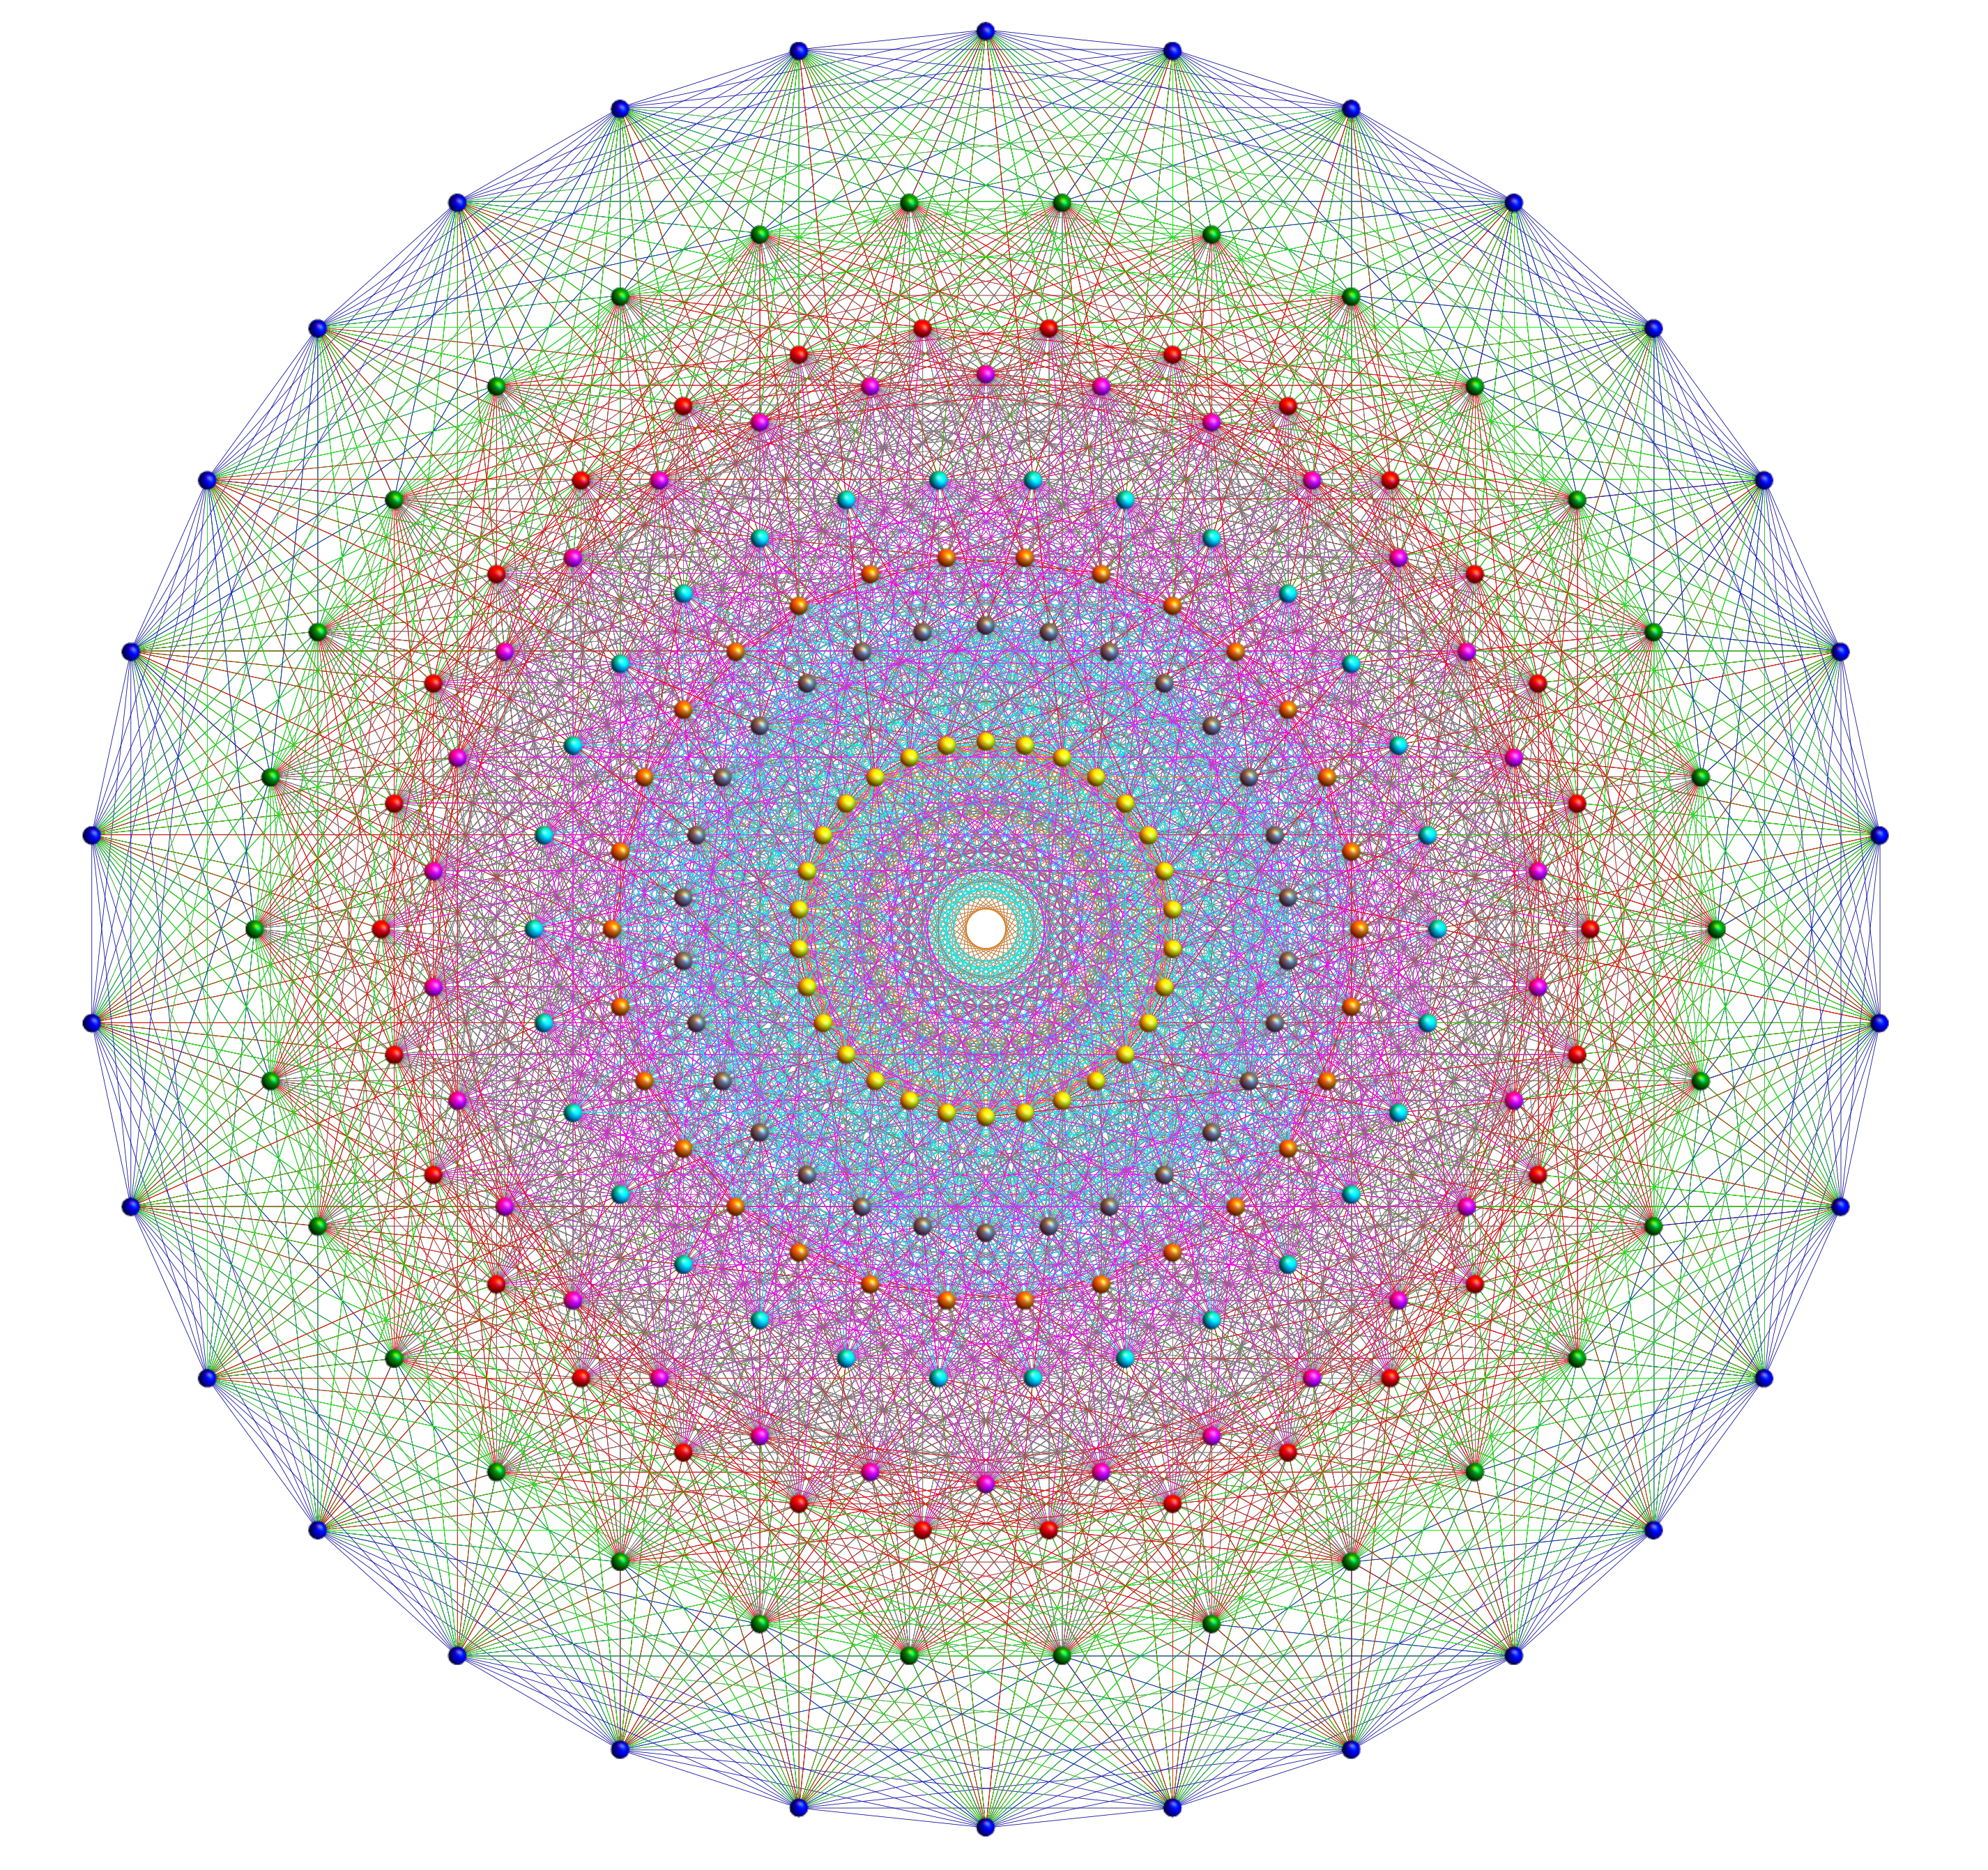
\includegraphics[width=1\columnwidth]{front.png}
\end{figure}
\newpage
\tableofcontents 
\newpage
\section{Calcolo differenziale in pi\`u variabili}
\subsection{Derivate parziali}

Una funzione di pi\`u variabili $f(x,y):\mathbb{R}^2 \to \mathbb{R}$ pu\`o essere derivata mantenendo fissa una variabile e derivando rispetto all'altra. Questo corrisponde al valutare la variazione di $f$ lungo un asse specifico.
\begin{definizione}
	{Derivata parziale}{}
	Sia $f(x_1,\ldots,x_n) :\mathbb{R}^n \to \mathbb{R}$; la sua derivata parziale rispetto a $x_k$ \`e:
	\begin{equation}
		\frac{\partial f}{\partial x_k}(x_1,\ldots,x_n) = \lim_{h \to 0} \frac{f(x_1,\ldots,x_k + h, \ldots, x_n)-f(x_1,\ldots,x_k,\ldots,x_n)}{h}
	\end{equation}
\end{definizione}
\noindent Il vettore che ha per componenti le derivate di $f$ rispetto a ciascuna delle sue variabili si chiama \textbf{gradiente} e si indica con $\nabla f$.

\subsection{Derivate direzionali}

\`E possibile studiare la variazione di $f$ lungo una particolare direzione individuata dal versore $\hat{n}$. Una retta parallela a $\hat{n}$ e passante per un punto $x$ si individua con $x+t \hat{n}$; fissando i punti $x$ e $\hat{n}$, $g(t) := f(x+t\hat{n})$ \`e una funzione di una variabile e $g'(0)$ \`e la derivata direzionale di $f$ lungo $\hat{n}$:
\begin{equation}
	\frac{\partial f}{\partial \hat{n}} (x) = g'(0) = \lim_{h \to 0} \frac{f(x+h\hat{n}) - f(x)}{h}
\end{equation}
Pi\`u in generale:
\begin{equation}
	g'(t) \overset{\text{def}}{=} \lim_{h \to 0} \frac{g(t+h) - g(t)}{h} = \lim_{h \to 0} \frac{f(x_t+ h \hat{n}) - f(x_t)}{h} \equiv \frac{\partial f}{\partial \hat{n}} (x_t)
\end{equation}
con $x_t = x+t \hat{n}$. 
\begin{obs}
	Conoscendo $\nabla f$, si pu\`o calcolare la derivata direzionale di $f$ come $\nabla f \cdot \hat{n}$.
\end{obs}
\begin{esempio}
	Si calcola la derivata direzionale di $f(x,y) = x^2 y - e^{x+y} $ lungo la direzione $\hat{n} = \left(\frac{1}{2}, \frac{\sqrt{3} }{2}\right) $.
	\begin{svolgimento}
		Si ha 
		\[
		g(t) = f\left(x + \frac{t}{2}, y + \frac{\sqrt{3} }{2}t\right) = \left(x + \frac{t}{2}\right) ^2 \left(y + \frac{\sqrt{3} }{2}t\right) - \exp \left[ x + y + t\left(\frac{1}{2} + \frac{\sqrt{3} }{2}\right)  \right] 
		\] 
		Allora 
		\[
		\frac{\partial f}{\partial \hat{n}} (x,y) = g'(0) = xy + \frac{\sqrt{3} }{2}x^2 - \left(\frac{1}{2}+ \frac{\sqrt{3} }{2} \right) e^{x+y} 
		\] 
		Alternativamente $\nabla f = \left(2xy - e^{x+y} , x^2 - e^{x+y} \right) $, quindi $\partial _{\hat{n}} f = \nabla f \cdot \hat{n} =xy - \frac{1}{2} e^{x+y} +\frac{\sqrt{3} }{2} x^2 - \frac{\sqrt{3} }{2}e^{x+y} = xy + \frac{\sqrt{3} }{2}x^2 - \left(\frac{1}{2}+\frac{\sqrt{3} }{2}\right) e^{x+y}   $.
	\end{svolgimento}
\end{esempio}
\begin{teorema}
	{}{}
	Se $f:A\subset \mathbb{R}^2 \to  \mathbb{R}$ ha un massimo o minimo relativo in $x_0$ interno ad $A$ e se ammette derivata lungo $\hat{n}$ in $x_0$, allora:
	\begin{equation}
		\frac{\partial f}{\partial \hat{n}} (x_0)= 0 
	\end{equation}
	\begin{proof}
		Si prende $g(t) = f(x_0 + t \hat{n})$ che, per costruzione, ha un minimo in $t=0$, quindi $g'(0) = 0$, da cui segue la tesi.
	\end{proof}
\end{teorema}
\noindent In particolare, se $f$ \`e derivabile in $x_0$, tutte le derivate parziali si annullano in quel punto; in questo caso, $x_0$ \`e detto \textbf{punto stazionario}.

\begin{obs}
	Nel caso a una variabile, i punti di massimo/minimo che cadevano sulla frontiera di un insieme erano, solitamente, un numero finito; qua chiaramente non \`e pi\`u cos\`i.
\end{obs}
\begin{esempio}
	Calcolare massimi e minimi di $f(x,y) = (x^2 + y^2 - 1)e^{x+y} $ nel cerchio chiuso centrato nell'origine e di raggio $1$.
	\begin{svolgimento}
		Sul bordo del cerchio $x^2 + y^2 = 1$, quindi $f\equiv 0$. All'interno:
		\[
			\begin{split}
				&f_x = 2x e^{x+y}  + (x^2 + y^2 -1)e^{x+y} \\
				&f_y = 2y e^{x+y} + (x^2 + y^2 - 1) e^{x+y} 
			\end{split}
		\] 
	che si annullano quando 
	\[
	\begin{split}
		&x^2 + y^2 + 2x - 1 = 0\\
		&x^2 + y^2 + 2y - 1 = 0
	\end{split}\Rightarrow 2x - 2y = 0 \Rightarrow x=y
	\] 
Sostituendo $x=y$ nella prima equazione, ad esempio, si ottengono due soluzioni, una sola delle quali appartiene al cerchio; questo corrisponder\`a al punto di minimo della funzione:
\[
f\left(\frac{\sqrt{3} -1}{2}, \frac{\sqrt{3} -1}{2}\right) = (1-\sqrt{3} ) e^{\sqrt{3} -1}  < 0
\] 
\end{svolgimento}
\end{esempio}
\noindent In pi\`u dimensioni vale un analogo del teorema di Lagrange:
\begin{teorema}
	{}{}
	Sia $f(x) : A \subset \mathbb{R}^n \to \mathbb{R}$ e $x_0 \in A$, con $I(x_0,r) \subset A$. Considerando una direzione $\hat{n}$, si definisce $g(s) = f(x_0+ s \hat{n})$ per $\lvert s \rvert <r$. Vale l'analogo del teorema di Lagrange:
	\begin{equation}
		f(x_0+s\hat{n}) - f(x_0) = g(s) - g(0) = s g'(\tau ) = s \frac{\partial f}{\partial \hat{n}} (x_0 + \tau \hat{n})
	\end{equation}
\end{teorema}

\subsection{Derivate successive}

Sia $f$ una funzione per cui esistono le derivate prime e sono anch'esse derivabili; le derivate seconde potranno essere derivate prima rispetto a $x_i$ e poi rispetto a $x_j$ o viceversa. In generale se $f$ \`e una funzione di $m$, si hanno $m^n$ derivate di ordine $n$. Per le derivate seconde miste\footnote{Chiaramente il risultato vale in generale, ma si affronta per funzione di due variabili nel caso delle derivate seconde miste per semplicit\`a.} vale il seguente.
\begin{teorema}
	{Teorema di Schwarz}{}
	Sia $f$ una funzione derivabile in un intervallo $I$ del punto $(x,y)$ e siano queste continue nello stesso intervallo; allora $f_{xy} (x,y) = f_{yx} (x,y)$.
	\begin{proof}
		Siano $h,k \in \mathbb{R}:(x+h,y+k) \in I$ e sia
		\[
		A(h,k) = f(x+h,y+k) - f(x+h,y) - f(x,y+k) + f(x,y)
		\] 
		Prendendo $p(t) = f(t,y+k) - f(t,y)$, si ha $A(h,k) = p(x+h) - p(x)$; per Lagrange:
		\[
			A(h,k) = p'(\xi ) h = \big[f_x(\xi ,y+k) - f_x(\xi ,y)\big]h ,\ x< \xi <x+h
		\] 
		Applicando nuovamente Lagrange, si ha $A(h,k) = f_{yx} (\xi, \eta) hk, \ y<\eta < y+k$. Ripetendo il discorso con $q(t) = f(x+h,t) - f(x,t)$, si trova $A(h,k) = f_{xy} (\sigma ,\tau ) hk$, quindi $f_{yx}(\xi ,\eta) =f_{xy} (\sigma ,\tau ) $, dove $x<\sigma <x+h$ e $y<\tau <y+k$. Prendendo il limite per $h,k\to 0$, risulta $f_{xy} (x,y) = f_{yx} (x,y)$ per continuit\`a delle derivate seconde.
		
	\end{proof}
\end{teorema}
\noindent Come per funzioni di una variabile, vale la formula di Taylor.
\begin{teorema}
	{Formula di Taylor}{}
	Sia $f(x)$ di classe $C^2$ in $A \subset \mathbb{R}^n$ e $x_0$ punto interno ad $A$; in un intorno di $x_0$, allora, si ha:
	\begin{equation}
		f(x) = f(x_0) + \left\langle \nabla f(x_0), x-x_0 \right\rangle + \frac{1}{2} \left\langle Hf(x_0) (x-x_0), x-x_0 \right\rangle + R_2(x;x_0)
	\end{equation}
	con 
	\[
	\lim_{x \to x_0} \frac{R_2(x;x_0)}{\left\lVert x-x_0 \right\rVert ^2} = 0
	\] 
	
\end{teorema}

\subsection{Funzioni differenziabili}


Una funzione derivabile, anche in ogni direzione, non \`e necessariamente continua in pi\`u variabili.
\begin{esempio}
	La funzione $f(x,y) = \begin{cases}
		\frac{xy^2}{x^2 + y^2}& , \ (x,y)\neq 0\\
		0 & , \ (x,y) =0 
	\end{cases}$ ha derivate in ogni direzione nel punto $(0,0)$, ma non \`e continua; prendendo $x_k = (1 / k , 1/k^2)$ per $k\to \infty$, si ha $x_k\to (0,0)$, ma $f(x_k) = \frac{1/k^4}{2 / k^4} \to \frac{1}{2}$.
\end{esempio}

\begin{definizione}{Differenziabilit\`a}{}
	Una funzione $f(x)$ si dice differenziabile in $x_0$ se \`e derivabile in $x_0 $ e se:
	\begin{equation}
		\lim_{x \to x_0} \frac{f(x) - f(x_0) - \langle \nabla f(x_0) , x -x_0 \rangle}{\left\lVert x - x_0 \right\rVert } = 0
	\end{equation}
\end{definizione}
\noindent Questa definizione impone che una funzione sia differenziabile in punto se esiste un piano tangente che la approssima precisamente nel punto stesso.

\begin{teorema}
	{}{}
	Una funzione $f(x)$ differenziabile in $x_0$ \`e continua in $x_0$ ed \`e derivabile in ogni direzione.
	\begin{proof}
		Si mostra che \`e continua:
		\[
		f(x) - f(x_0)  = \frac{f(x) - f(x_0) - \langle \nabla f(x_0) , x-x_0 \rangle}{\left\lVert x-x_0 \right\rVert } \left\lVert x-x_0 \right\rVert + \langle \nabla f(x_0) , x-x_0 \rangle
		\] 
		Per $x\to x_0$ il primo termine di destra va a $0$ per assunzione di differenziabilit\`a e l'altro anche perch\'e diventa un prodotto scalare per $0$, quindi si verifica $\lim_{x \to x_0} f(x) = f(x_0)$.

		Data generica direzione $\hat{v}$ con $x = x_0 + t \hat{v}$, usando ancora definizione di differenziabilit\`a:
		\[
		\lim_{t \to 0} \frac{f(x_0 + t \hat{v})- f(x_0) - \langle \nabla f(x_0), t \hat{v} \rangle}{t} = 0 
		\] 
Visto che $\langle \nabla f(x_0 ) , t \hat{v} \rangle = t \langle \nabla f(x_0) ,\hat{v} \rangle$, si ottiene la tesi.
	\end{proof}
\end{teorema}
\noindent La direzione di massimo incremento di una funzione \`e quella del gradiente. Per mostrarlo, si parte da $x_0$, assumendo che non sia un punto stazionario; si definisce, allora, $\hat{n} = \frac{\nabla f(x_0)}{\left\lVert \nabla f(x_0) \right\rVert} $, da cui:
\[
\frac{\partial f}{\partial \hat{n}} (x_0) = \langle \nabla f(x_0), \hat{n} \rangle = \left\lVert \nabla f(x_0) \right\rVert 
\] 
Prendendo altra direzione generica $\hat{v}$, si ha:
\[
\frac{\partial f}{\partial \hat{v}} (x_0) = \langle \nabla f(x_0) , \hat{v}  \rangle \le  \left\lVert \nabla f(x_0) \right\rVert \left\lVert \hat{v} \right\rVert = \left\lVert \nabla f(x_0) \right\rVert \equiv \frac{\partial f}{\partial \hat{n}} (x_0)
\] 
Dalla definizione di funzione differenziabile il piano $z = f(x_0,y_0) +f_x(x_0,y_0) (x-x_0) + f_y(x_0,y_0) (y-y_0)$ \`e quello che meglio approssima la funzione in $(x_0,y_0)$.

Si \`e concluso che una funzione differenziabile \`e derivabile in ogni direzione, ma una funzione derivabile non \`e differenziabile in generale. Vale, per\`o, il seguente.
\begin{teorema}
	{Teorema del differenziale totale}{}
	Sia $f(x)$ derivabile in $x_0$ e siano le sue derivate continue nello stesso punto; allora $f$ \`e differenziabile in $x_0$.
	\begin{proof}
		Si vuole dimostrare che
		\[
		\lim_{(x,y) \to (x_0,y_0)} \frac{f(x,y) - f(x_0,y_0) - f_x(x_0,y_0) (x-x_0) - f_y(x_0,y_0)(y-y_0)}{\sqrt{(x-x_0)^2 + (y-y_0)^2} } = 0
		\] 
		Si usa il teorema di Lagrange per riscrivere $f(x,y) - f(x_0,y_0)$:
		\[
		\begin{split}
			&f(x,y_0) - f(x_0,y_0) = f_x(\xi ,y_0) (x-x_0),\ x_0<\xi <x\\
			&f(x,y) - f(x,y_0) = f_y(x ,\eta) (y-y_0), \ y_0 < \eta < y\\
			&\Rightarrow f(x,y) - f(x_0,y_0) = f_x(\xi ,y_0) (x-x_0) + f_y(x,\eta) (y-y_0)
		\end{split}
		\] 
	Il limite scritto sopra si riscrive come:
	\[
		\begin{split}
			\lim_{(x,y) \to (x_0,y_0)} \big[f_x(\xi ,y_0) - f_x(x_0,y_0)\big] &\frac{x-x_0}{\sqrt{(x-x_0)^2 + (y-y_0)^2} } + \\ 
											  &+\big[f_y(x,\eta) - f_y(x_0,y_0)\big] \frac{y-y_0}{\sqrt{(x-x_0)^2 + (y-y_0)^2} }
		\end{split}
	\] 
	Essendo le frazioni $\le 1$ e visto che le quantit\`a fra parentesi quadre, questo limite si maggiora con la somma delle parentesi quadre, che tende a $0$ per $(x,y) \to (x_0,y_0)$.
	\end{proof}
\end{teorema}
\subsection{Funzioni composte}
	Data una funzione $x(t) : \mathbb{R}^k \to \mathbb{R}^n$, si definisce, per una generica direzione $v$:
	\begin{equation}
		\frac{\partial x}{\partial v} = \left(\frac{\partial x_1}{\partial v}, \ldots , \frac{\partial x_n}{\partial t}  \right) ^\top
	\end{equation}
Vale il seguente per la derivata della funzione composta.
\begin{teorema}
	{}{}
	Siano $E \subset  \mathbb{R}^k , \ F \subset \mathbb{R}^n$ e $x(t) : E \to F , \ f(x) : F \to \mathbb{R}$ funzioni di classe $C^1$. Allora la funzione composta $g(t) = f(x(t)) : E \to\mathbb{R}$ \`e di classe $C^1$ e per ogni direzione $v$:
	\begin{equation}
		\frac{\partial g}{\partial v} (t) =\left\langle \nabla f\big(x(t)\big), \frac{\partial x}{\partial v} (t) \right\rangle
	\end{equation}
	\begin{proof}
		Si ha $g(t + h v) -g(t) = f\big(x(t+hv)\big) - f\big(x(t)\big) = f\big(x(t) + [x(t+hv) - x(t)]\big) - f\big(x(t)\big)$. Si prende $s = \lVert x(t+hv) - x(t) \rVert $ e la direzione$w = \frac{x(t+hv) - x(t)}{s}$ e si usa il teorema di Lagrange:
		\[
		g(t+hv) - g(t) = f\big(x(t) + s w\big) - f\big(x(t)\big) = s \frac{\partial f}{\partial w} \big(x(t) + \tau w\big) = s \left\langle \nabla f \big(x(t) + \tau  w\big), w \right\rangle
		\] 
	con $0<\tau <s$. Dividendo per $h$ e prendendo il limite $h\to 0$, per definizione $s \to 0$ e, quindi, $\tau  \to 0$, mentre $\frac{x(t+hv) - x(t)}{h}\to \frac{\partial x}{\partial v} (t)$ quindi:
\[
\lim_{h \to 0} \frac{g(t+ hv) -g(t)}{h} = \lim_{h \to 0} \left\langle \nabla f\big(x(t) + \tau  w\big), \frac{x(t+hv) - x(t)}{h} \right\rangle = \left\langle\nabla f\big(x(t)\big), \frac{\partial x}{\partial v} (t)  \right\rangle
\] 
	\end{proof}
\end{teorema}
\noindent Nel caso particolare $k=1$, $x(t)$ \`e una curva e $g(t)$ \`e funzione di una sola variabile con
\[
g'(t) = \sum_{h=1}^{n} \frac{\partial f}{\partial x_h} \big(x(t)\big) x'_h(t) \equiv \Big\langle \nabla f \big(x(t)\big), x'(t) \Big\rangle
\] 
Spesso si prende $x(t) = x + t v $, cio\`e retta passante per $x$ lungo direzione $v$; in questo caso $g'(t) = \nabla f(x+tv) \cdot  v$. Se le derivate seconde sono continue, le derivate prime sono differenziabili e si pu\`o scrivere:
\begin{equation}
	g''(t)	= \sum_{i=1}^{n} v_i \frac{d }{d t} D_i f (x+tv) = \sum_{i=1}^{n} v_i \sum_{j=1}^{n} v_j D_{ij} f(x+tv)
\end{equation}
Indicando con $Hf = \nabla f \nabla ^\top$ la matrice Hessiana di $f$, allora $\sum_{j}^{} v_j D_{ij} f(x+tv) \equiv \left[ Hf(x+tv) v\right]_i $, cio\`e \`e la componente $i$-esima del vettore tra parentesi quadre, essendo $Hf$ una matrice. Allora:
\begin{equation}
	\begin{split}
		&g'(0) = \nabla f(x) \cdot v \\ 
		& g''(0) = \langle Hf(x) v , v \rangle
	\end{split}
\end{equation}
 
\subsection{Massimi e minimi relativi}

Perch\'e una funzione $f$ di pi\`u variabili abbia un punto di massimo o di minimo in $x_0$, \`e condizione necessaria che per ogni direzione $v$, valga $g'(0) = 0$ e $g''(0) \le 0$ o $g''(0) \ge 0$, cio\`e:
\begin{equation}
	\begin{split}
		&\langle Hf (x_0) v , v \rangle \le 0 \text{ punto di massimo}\\
		&\langle Hf (x_0) v , v \rangle \ge 0 \text{ punto di minimo}
	\end{split}
\end{equation}
Allora vale il seguente.
\begin{teorema}
	{}{}
	Sia $f(x)$ una funzione con derivate seconde continue; se in $x_0$, $\nabla f (x_0) = 0$ e la matrice Hessiana \`e tale che $Hf(x_0) > 0$ (definita positiva), allora $x_0$ \`e di minimo relativo per $f$. Se fosse $Hf(x_0) < 0$, $x_0$ sarebbe di massimo relativo.
\end{teorema}
\noindent Possono verificarsi altri due casi:
\begin{itemize}
	\item se $\langle H f(x_0)v ,v \rangle $ assume sia valori positivi che negativi al variare di $v$, si ha un \textbf{punto di sella};
	\item se la matrice Hessiana \`e semidefinita, ma non definita, non si pu\`o concludere niente e bisogna esaminare cosa accade attorno a $x_0$.
\end{itemize}

\newpage 

\section{Calcolo integrale in pi\`u variabili}

\subsection{Integrazione in dimensioni superiori}
Per le definizioni di base, si deve definire cos'\`e un rettangolo.
\begin{definizione}
	{}{}
	Dati due intervalli $[a.b)$ e $[c,d)$, il rettangolo che identificano \`e definito come $R = [a,b) \times  [c,d)$, con $a\le x< b$ e $c\le y<d$.
\end{definizione}
\noindent Si suddividono due intervalli in intervalli pi\`u piccoli, cio\`e $[a,b)$ si suddivide in $n$ sotto-intervalli $I_h = [x_{h-1} ,x_h)$, con $x_0 =a , \ldots x_n = b$ e $[c,d)$ in $m$ sotto-intervalli $J_k = [y_{k-1} ,y_k)$. Allora il rettangolo sar\`a suddiviso in $n\times m$ sotto-rettangoli $R_{hk}  = I_h \times J_k$.

Una funzione semplice $\varphi (x)$ \`e una funzione che assume un valore costante su ogni sotto-rettangolo e che vale $0$ fuori da $R$. Indicando con $\lambda _{hk}$ il valore costante che assume in $R_{hk} $:
\begin{equation}
	\varphi (x)= \sum_{h=1}^{n} \sum_{k=1}^{m} \lambda _{hk} \chi _{R_{hk} } (x)
\end{equation}
con $\chi _D$ funzione caratteristica del dominio $D$. L'integrale di funzioni simili \`e dato da:
\begin{equation}
	\int \varphi (x) \ dxdy = \sum_{h=1}^{n} \sum_{k=1}^{m} \lambda _{hk} m(R_{hk} )= \sum_{h=1}^{n} \sum_{k=1}^{m} \lambda _{hk} m(I_h) m(J_k) = \sum_{h=1}^{n} \sum_{k=1}^{m} \lambda _{hk} (x_h -x_{h-1} ) (y_k - y_{k-1} )
\end{equation}
\`E necessario dare anche la definizione di supporto di una funzione:
\begin{definizione}
	{}{}
	Il supporto di una funzione $f$ \`e la chiusura dell'insieme in cui $f\neq 0$, cio\`e:
	\begin{equation}
		\operatorname{supp} (f) = \overline{\left\{ x : f(x) \neq 0 \right\} }
	\end{equation}
\end{definizione}
\noindent Infine, si indica con $\mathscr{S}^+(D)$ la classe delle funzioni semplici $\varphi $ che maggiorano $f$ in $D$ e $\mathscr{S}^-(D)$ la classe delle funzioni semplici $\psi $ che minorano $f$ in $D$; da questo, si ha la seguente definizione di integrale di Riemann.
\begin{definizione}
	{Integrazione di funzioni a supporto compatto}{}
	Sia $f$ una funzione a supporto compatto, con $\operatorname{supp} (f) \subset K$; $f$ \`e integrabile secondo Riemann se:
	\begin{equation}
		\sup_{\psi \in \mathscr{S}^-(K)}  \int \psi  \ dx dy = \inf_{\varphi \in \mathscr{S}^+(K)}  \int \varphi \ dxdy
	\end{equation}
	dove
	\begin{equation}
		\begin{split}
			&\int_{*} f(x) \ dx =  \inf_{\varphi \in \mathscr{S}^+(K)}  \int \varphi \ dxdy \ \text{ integrale inferiore} \\
			&\int^{*} f(x) \ dx =  \sup_{\psi  \in \mathscr{S}^-(K)}  \int \psi  \ dxdy \ \text{ integrale superiore} \\
		\end{split}
	\end{equation}
	La condizione di integrabilit\`a si pu\`o esprimere come:
	\begin{equation}
		\int_{*} f(x) \ dx= \int^{*} f(x) \ dx
	\end{equation}
\end{definizione}
\begin{obs}
	Anche per pi\`u variabili, \`e condizione sufficiente e necessaria perch\'e $f$ a supporto compatto sia integrabile che $\forall \varepsilon >0$, esistono funzioni semplici $\varphi ,\psi $ tali che:
	\begin{equation}
		\int \varphi  \ dxdy - \int \psi  \ dxdy < \varepsilon 
	\end{equation}
\end{obs}
\subsection{Misura di insiemi}
L'integrabilit\`a di una funzione su un certo insieme $E$ \`e legata alla misura dell'insieme stesso.
\begin{definizione}
	{Misurabilit\`a di insiemi}{}
	Un insieme $E$ \`e \textit{misurabile} (secondo Peano-Jordan) se la sua funzione caratteristica $\varphi _E$ \`e integrabile. In questo caso, la misura \`e:
	\begin{equation*}
		m(E) = \int \varphi _E \ d\mathbf{x} 
	\end{equation*}
\end{definizione}
\noindent Se $\varphi _E$ \`e integrabile, allora $\forall \varepsilon >0$, si avrebbero $\psi ,\varphi $ funzioni semplici con $\psi \le  \varphi _E \le \varphi $ tali che:
\[
\int \varphi  \ d\mathbf{x}  - \int \psi \ d\mathbf{x} < \varepsilon 
\] 
L'idea \`e suddividere il piano $x,y$ in rettangoli $R_{hk} $ dove $\varphi =1$ nei rettangoli $R_{hk} $ che hanno punti in comune con $E$ ed \`e nulla negli altri, mentre si prende $\psi =1 $ nei rettangoli contenuti in $E$ e pari a $0$ negli altri. Cos\`i facendo, l'integrale di $\varphi $ \`e la somma delle misure dei rettangoli $R_{hk}$ che hanno punti in comune con $E$, mentre quello di $\psi $ \`e la somma delle misure degli $R_{hk} $ contenuti in $E$. Il risultato della differenza \`e la somma delle misure dei rettangoli che hanno punti in comune con $E$, ma che non vi sono contenuti, quindi sar\`a la somma delle misure dei rettangoli che hanno punti in comune con la frontiera di $E$.

Si definisce \textbf{plurirettangolo} l'unione $P$ di un numero finito di rettangoli senza punti comuni, la cui misura coincide con la somma delle misure dei rettangoli che lo compongono; si ha la seguente.
\begin{prop}
	{}{mis21}
	Un insieme $E$ \`e misurabile $\iff \forall \varepsilon >0, \ \exists $ un plurirettangolo $P$ contenuto in $E$ e un plurirettangolo $Q$ che contiene $E$ tali che $m(Q) - m(E) < \varepsilon $.
\end{prop}
\noindent Usando Prop \ref{prop:mis21}, se $P,Q$ plurirettangoli t.c. $P \subset E \subset Q$, con $m(Q-P) = m(Q) - m(P)$, si ha che:
\begin{center}
	\textit{Un insieme $E$ \`e misurabile $\iff \forall \varepsilon > 0$ esiste $Z$ plurirettangolo che contiene $\partial E$, con $m(Z)<\varepsilon $.} 
\end{center}
Quindi:
\begin{center}
	\textit{Un insieme $E$ \`e misurabile (secondo Peano-Jordan) $\iff$ la sua frontiera\newline $\partial E$ ha misura nulla.} 
\end{center}
\begin{prop}
	{}{}
	Se due insiemi $A,B$ sono misurabili, allora sono misurabili anche $A \cup B , \ A \cap B $ e $A \setminus B$.
	\begin{proof}
		$A,B$ misurabili $\implies$ $\partial A, \ \partial B$ sono contenute in plurirettangoli $Z_A,Z_B$ che hanno misura minore di $\varepsilon , \ \forall \varepsilon >0$, quindi $m(Z_A \cup Z_B) < 2 \varepsilon $. Questo vuol dire che $m(\partial A \cup \partial B) = 0$, quindi le frontiere di $A\cup B , \ A \cap B $ e $A \setminus B$ hanno misura nulla.
	\end{proof}
\end{prop}
\subsubsection{Insiemi generati da funzioni}
Siano $g(x):\left[ a,b \right] \subset \mathbb{R} \to \mathbb{R}^{\ge 0}  $  e $G:= \left\{ (x,y) \in \mathbb{R}^2 : a\le x\le b , \ 0 \le  y \le  g(x) \right\}$. Se $g$ \`e integrabile, l'insieme $G$ \`e misurabile, con 
\begin{equation}
	m(G) = \int_{a} ^b g(x) \ dx
\end{equation}
\begin{proof}
	Essendo $g$ integrabile, $\forall \varepsilon >0$, esistono $\varphi ,\psi $ con $\int (\varphi -\psi ) \ dx < \varepsilon  $. Considerando i plurirettangoli 
	\[
		\Phi := \left\{ (x,y) \in \mathbb{R}^2 : a\le x\le b , \ 0\le  y \le \varphi (x) \right\} \hspace{.1cm} , \hspace{.2cm} \Psi := \left\{ (x,y) \in \mathbb{R}^2 : a\le x\le b , \ 0\le  y \le \psi (x) \right\}
	\] 
	per i quali
	\[
		m(\Phi) = \int \varphi  \ dx \hspace{.1cm} , \hspace{.2cm} m(\Psi) = \int \psi  \ dx 
	\] 
	si ha $\Psi \subset G \subset \Phi$ con $m(\Phi) - m(\Psi) < \varepsilon \Rightarrow G$ misurabile. 
	Inoltre, per quanto detto, sia $m(G)$ che $\int g \ dx$ sono contenuti tra $m(\Phi)$ e $m(\Psi)$, cio\`e:
	\[
	\left\lvert m(G) - \int_{a} ^b g(x) \ dx \right\rvert < m(\Phi) - m(\Psi)  < \varepsilon , \ \forall \varepsilon \implies m(G) = \int_{a} ^b g(x) \ dx
	\] 
	
\end{proof}
Siano, ora, $g,h$ due funzioni integrabili in $[a,b)$ con $0\le g(x) \le  h(x)$. L'insieme $E:=\left\{ (x,t) \in \mathbb{R}^2 : a\le x\le b, \ g(x) \le y \le h(x) \right\} $ \`e misurabile per quanto detto sopra, essendo $E$ dato dalla differenza degli insiemi $H,G$ definiti come sopra e misurabili a loro volta. Inoltre, sempre applicando quanto detto sopra alla differenza di $H,G$:
\[
m(E) = \int_{a} ^b \left[ h(x) - g(x) \right] \ dx 
\] 
\begin{obs}
	Questo \`e valido anche per $g,h$ non-positive; \`e, infatti, sufficiente applicare il ragionamento alle funzioni $h+c, \ g+c$, con $c$ preso in modo che siano entrambe positive e osservando che $E_c$ corrisponde a $E$ traslato di $c$ verso l'alto.
\end{obs}
\subsection{Integrabilit\`a di funzioni continue}
\begin{teorema}
	{}{}
	Sia $f(\mathbf{x} )$ continua in rettangolo chiuso $R$ e sia $E$ un insieme misurabile con $E \subset R$. Allora $f$ \`e integrabile in $E$.
	\begin{proof}
	Si mostra che $f \varphi _E$ \`e integrabile. 
	Per Weierstrass, $f$ \`e uniformemente continua in $R$, quindi $\forall \varepsilon >0, \ \exists \delta (\varepsilon )>0$ t.c. la divisione di $R$ in rettangoli $R_{hk} $ di diametro minore di $\delta (\varepsilon )$, risulta:
	\[
	M_{hk } - m_{hk}  = \sup_{R_{hk} } f - \inf_{R_{hk} } f < \varepsilon 
	\] 
Inoltre, $f$ ha massimo e minimo in $R$, indicati, rispettivamente, con $M$ e $m$. 
Allo stesso tempo, $E$ \`e misurabile, quindi $\forall \varepsilon >0, \ \exists $ suddivisione di $R$ in $R_{hk} $, assunta di diametro inferiore di $\delta (\varepsilon )$, tale che la misura dei rettangoli che hanno almeno un punto in comune con $\partial E$ \`e minore di $\varepsilon $.

Con questa suddivisione, si classificano con $\mathcal{I}, \mathcal{E}, \mathcal{F}$ rispettivamente i rettangoli interni, esterni e a contatto con la frontiera di $E$. Per la misurabilit\`a di $E$:
\[
\sum_{R_{jk} \in \mathcal{F}}^{} m(R_{hk} ) < \varepsilon 
\] 
Si definiscono:
\begin{itemize}
	\item funzione maggiorante $\varphi  $ che \`e nulla nei rettangoli esterni, $\phi = \max\left\{ M,0 \right\} $ in quelli di frontiera e $\phi = M_{hk} $ in quell interni.
	\item funzione minorante $\psi $ che \`e nulla in quelli esterni, $\psi = \min\left\{ m , 0 \right\} $ in quelli di frontiera e $\psi  = m_{hk} $ in quelli interni.
\end{itemize}
Quindi $\psi \le f\varphi  _E \le \varphi $ e
\[
\begin{split}
	\int (\varphi-\psi )  \ dx dy&= \big(\max \left\{ M,0 \right\} - \min \left\{ m,0 \right\} \big) \sum_{R_{hk} \in \mathcal{F}}^{} m(R_{hk}) + \sum_{R_{hk} \in \mathcal{I}}^{} (M_{hk} -m_{hk} ) m(R_{hk}) \\
						   &< \left(\lvert M \rvert +\lvert m \rvert \right) \varepsilon  + \varepsilon \sum_{R_{hk} \in \mathcal{I}}^{} m(R_{hk} ) < \varepsilon \big(\lvert M \rvert +\lvert m \rvert +m(R)\big) 
\end{split}
\] 
Allora $f$ \`e integrabile su $E$.
\end{proof}
\end{teorema}
\noindent Pi\`u in generale, vale il seguente.
\begin{teorema}
	{}{}
	Sia $f$ limitata in un rettangolo $R$. Questa \`e integrabile in $E\subset R$ se l'insieme $D$ dei suoi punti di discontintui\`a ha misura nulla.
	\begin{proof}
		Si ripete la dimostrazione precedente con $D$ al posto di $\partial E$.
	\end{proof}
\end{teorema}
\subsection{Integrali doppi}
Si analizza prima caso per funzioni semplici. 
Si considera suddivisione del rettangolo $R=I\times J$ in rettangoli $R_{hk} = I_h \times J_k$.
Sia $\varphi = \sum_{}^{} \lambda _{hk}\varphi _{R_{hk} } $ funzione semplice; fissando $x \in I_h$, si considera $\varphi $ come funzione della sola $y$ e:
\[
\int \phi (x,y) \ dy = \sum_{k}^{} \lambda _{hk} m(J_k)
\]
L'integrale a primo membro \`e costante per $x \in I_h$, pertanto \`e a sua volta una funzione semplice; integrandolo rispetto a $x$:
\[
\int dx \int \phi (x,y) \ dy = \sum_{h}^{} m(I_h) \sum_{k}^{} \lambda _{hk} m(J_k)= \sum_{h,k}^{} \lambda _{hk} m(I_h)m(J_k) = \sum_{h,k}^{} \lambda _{hk} m(R_{hk} )= \int\varphi  \ dxdy
\] 
Il discorso \`e analogo integrando prima rispetto a $x$ e poi rispetto a $y$. 
Si generalizza con il seguente.
\begin{teorema}
	{Teorema di Fubini}{}
	Sia $f(x,y)$ integrabile in $R = [a,b) \times [c,d)$ e sia questa integrabile $\forall x \in [a,b)$ rispetto alla variabile $y \in [c,d)$. 
	Allora la funzione $F(x) = \int_{c} ^d f(x,y) \ dy$ \`e integrabile in $[a,b)$ e 

	\[
	\int_{R} f(x,y) \ dxdy = \int_{a} ^b F(x) \ dx = \int_{a} ^b dx \int_{c} ^d f(x,y) \ dy
	\] 
\begin{proof}
	Visto che $f$ \`e integrabile in $R$, allora esistono $\psi , \varphi $ funzioni semplici t.c.
	\[
	\psi \le f \varphi _R \le \varphi, \text{ con }   \int (\varphi -\psi ) \ dxdy < \varepsilon 
	\] 
	Integrando le disuguaglianze rispetto alla $y$, si ottiene:
	\begin{equation}\label{ftheq1}
	\Psi(x) = \int_c^d \psi \ dy \le F(x) = \int_{c} ^d f\ dy \le \int_{c} ^d \varphi \ dy = \Phi(x)
	\end{equation}
	Le funzioni $\Phi,\Psi$ sono ancora funzioni semplici, rispettivamente maggiorante e minorante di $F$, per le quali vale
	\[
	\int_{a} ^b (\Phi-\Psi) \ dx = \int (\varphi -\psi ) \ dxdy < \varepsilon 
	\] 
	Quindi $F(x)$ \`e integrabile in $[a,b)$.
	Ora, integrando in $[a,b)$ l'eq. \ref{ftheq1}, si ha:
	\[
	\int_{R} \psi  \ dxdy \le \int_{a} ^b F(x) \ dx \le  \int_{R} \varphi (x,y) \ dxdy
	\] 
	Allo stesso tempo, integrando la disuguaglianza iniziale su $R$:
	\[
	\int_{R} \psi  \ dxdy \le \int_{R} f \ dxdy \le \int_R \varphi  \ dxdy
	\] 
	Unendo le due disuguaglianze:
\[
\left\lvert \int_{R} f(x,y)\ dxdy - \int_{a} ^b F(x) \ dx \right\rvert \le \int_{R} (\varphi -\psi ) \ dxdy < \varepsilon
\] 
Valendo $\forall \varepsilon >0$, si ottiene la tesi.
\end{proof}	
\end{teorema}
\noindent Questo teorema si applica anche a integrali su \textit{insiemi normali rispetto all'asse} $y$\footnote{Insiemi, la cui intersezione con la retta verticale $x=\text{cost.}$ \`e un segmento o un punto.}
\[
E := \left\{ (x,y) \in \mathbb{R}^2 : a\le x\le b , \ g(x) \le  y \le h(x) \right\} 
\] 
con $g,h$ continue in $[a,b]$. Per quanto visto, $E$ \`e misurabile e, se $f$ \`e continua su $E$, \`e anche integrabile in $E$ stesso. 
In generale, la funzione $f^* = f \varphi _E$ \`e integrabile in ogni rettangolo $R = [a,b] \times  [c,d] \supset E$.

Fissata $x \in [a,b)$, la funzione $f^*(x,y)$ vale $f(x,y)$ se $g(x) \le  y \le h(x)$ e $0$ altrimenti, quindi \`e continua tranne, al pi\`u, nei punti $g(x), h(x)$. Allora $f^*$ \`e integrabile e si pu\`o applicare Fubini:
\[
	\int_{R} f^*(x,y) \ dxdy = \int_{a} ^b dx \int_{c} ^d f^*(x,y) \ dy \implies \int_{E} f \ dxdy = \int_{a} ^b dx \int_{g(x)} ^{h(x)} f \ dy
\] 
\begin{esempio}
Calcolare
\[
\int_{E} x^2 y \ dxdy, \ E := \left\{ (x,y) \in \mathbb{R}^2:-1\le x\le 1 , \ 0 \le  y \le  \sqrt{1-x^2}  \right\} 
\] 
con $E$ semicirconferenza di raggio $1$ e centro l'origine.
\begin{svolgimento}
	L'insieme \`e normale rispetto all'asse $y$ e, per Fubini:
	\[
	\begin{split}
		\int_E x^2  y \ dxdy &= \int_{-1} ^{+1} dx \int_{0} ^{\sqrt{1-x^2} } x^2 y \ dy = \frac{1}{2}\int_{-1} ^{+1} \left[ x^2 y^2 \right] _{0} ^{\sqrt{1-x^2} }  dx\\
				     &= \frac{1}{2}\int_{-1} ^{+1} x ^2 (1-x^2) \ dx = \Eval{\left(\frac{x^3}{6}- \frac{x^5}{10}\right) }{-1}{+1} = \frac{2}{15}
	\end{split}
	\] 
	
\end{svolgimento}
\end{esempio}
\subsection{Integrali tripli}
Il teorema di Fubini si applica anche nel caso di tre o pi\`u variabili: se $f(x,y,z)$ \`e integrabile nel parallelepipedo $P = [a,b) \times [c,d) \times [r,s)$ e, $\forall (x,y) \in R = [a,b) \times [c,d)$, \`e integrabile rispetto a $z$, allora:
\[
\int_{P} f(x,y,z) \ dxdydz = \int_{R} dxdy \int_{r} ^s f(x,y,z) \ dz
\] 
In particolare, se $f$ \`e continua in $E$ insieme normale rispetto a $z$, cio\`e della forma $E:= \left\{ (x,y,z) \in \mathbb{R}^3 : (x,y) \in R, \ g(x,y)\le z \le h(x,y) \right\} $, si ha:
\begin{equation}\label{volintfub}
	\int_{E} f(x,y,z) \ dxdydz = \int_{R} dxdy \int_{g(x,y)} ^{h(x,y)} f(x,y,z) \ dz
\end{equation}
Ovviamente il ragionamento si pu\`o poi applicare quando si dovr\`a calcolare l'integrale doppio.
\begin{esempio}
Per $E:=\left\{ (x,y,z) \in \mathbb{R}^3 : x>0,y>0,z>0, \ x+y+z < 2\right\} $, calcolare
\[
\int_{E} (x+y-z) \ dxdydz
\] 
\begin{svolgimento}
	L'insieme \`e normale rispetto a $z$, quindi:
	\[
	\int_{E} (x+y-z) \ dxdydz = \int_{T} dxdy \int_{0} ^{2-x-y}  (x+y-z) \ dz
	\] 
	con $T:= \left\{ (x,y) \in \mathbb{R}^2:x>0,y>0, \ x+y <2 \right\} = \left\{ (x,y) \in \mathbb{R}^2 : 0<x<2, \ 0<y<2-x \right\}  $. 
	L'ultimo integrale \`e:
	\[
	\int_{0} ^{2-x-y} (x+y-z) \ dz = \left[ xz + yz - \frac{z^2}{2} \right] _{0} ^{2-x-y}  = 4(x+y) - \frac{3}{2}(x+y)^2 - 2
	\] 
	L'integrale doppio rimanente si pu\`o nuovamente spezzare con Fubini:
	\[
	\begin{split}
		\int_{T} \left[ 4(x+y) - \frac{3}{2}(x+y)^2 - 2\right]  dxdy &= \int_{0} ^2 dx \int_{0} ^{2- x} \left[ 4(x+y) - \frac{3}{2}(x+y)^2 - 2\right] dy\\
									     &=\int_{0} ^2 \left[ 4xy + 2y^2 - \frac{3}{2}\left(x^2 y + xy^2  + \frac{1}{3}y^3\right) -2y \right] _{y=0} ^{y= x-2} dx \\
									     &=\int_{0} ^2 \left(\frac{1}{2}x^3 - 2 x^2 + 2x\right) dx = \left[ \frac{1}{8} x^4 - \frac{2}{3}x^3 + x^2\right] _0^2= \frac{2}{3}
	\end{split}
	\] 
	
\end{svolgimento}
\end{esempio}
\noindent L'eq. \ref{volintfub} si pu\`o usare nel calcolo di volumi degli insiemi normali. Dato 
\[
E := \left\{ (x,y,z) \in \mathbb{R}^3 : (x,y) \in F, \ g(x,y) \le z \le h(x,y) \right\} 
\] 
e posto $f=1$ in eq. \ref{volintfub}, si ha:
\begin{equation}\label{misfub}
	m(E) = \int_{F} \big[h(x,y) - g(x,y)\big] dxdy
\end{equation}
\begin{esempio}
Per $Q = (0,1) \times (0,1)$, calcolare il volume dell'insieme
\[
	E := \left\{ (x,y,z) \in \mathbb{R}^3 : (x,y) \in Q, \ x+y \le z \le  x^2 + y^2 + 1 \right\} 
\] 
\begin{svolgimento}
	Usando direttamente eq. \ref{misfub}, si ha:
	\[
		\begin{split}
			m(E) &= \int_{Q} (1+x^2 + y^2 - x - y) dxdy = \int_{0} ^1 dy \int_{0} ^1 (1+x^2 + y^2 -x - y) dx \\
			     &= \int_{0} ^1 \left(1+ \frac{1}{3}  + y^2 - \frac{1}{2} - y\right) dy = \frac{2}{3}
		\end{split}
	\] 
	
\end{svolgimento}
\end{esempio}
\subsection{Cambiamento di variabili}
Si inizia con il caso di $f(x,y)$ funzione di due variabili, integrabile e a supporto compatto.
Nell'ipotesi che valga il teorema di Fubini:
\[
\int f(x,y) \ dxdy = \int dx \int (x,y) \ dy
\] 
Si fissa $x$ nell'ultimo integrale e si cambia variabile con $y= \varphi (x,v)\Rightarrow dy = \varphi _v (x,v) dv $, da cui
\[
\int f(x,y) \ dxdy = \int dx \int f\big(x,\varphi (x,v)\big)\lvert \varphi _v(x,v) \rvert dv
\] 
Usando il teorema di Fubini due volte, si pu\`o scrivere l'ultimo integrale prima come integrale doppio e poi come integrale prima rispetto a $x$ e poi rispetto a $v$:
\[
\int f(x,y) \ dxdy = \int f\big(x,\varphi (x,v)\big) \lvert \varphi (x,v) \rvert  \ dxdv  = \int dv \int f\big(x,\varphi (x,v)\big)\lvert \varphi _v(x,v) \rvert  dx
\] 
Nell'ultimo integrale, si fissa $v$ e si cambia variabile con $x=x(u,v)\Rightarrow dx = x_u (u,v) du$:
\[
\int f(x,y) \ dxdy = \int dv \int f\Big(x(u,v) , \varphi \big(x(u,v), v\big)\Big) \left\lvert \varphi _v\big(x(u,v) , v\big) x_u(u,v)\right\rvert du
\] 
Infine, si prendono:
\[
\begin{cases}
	x = x(u,v)\\
	y=\varphi \big(x(u,v),v\big)=y(u,v)
\end{cases}\implies \begin{cases}
y_u(u,v) = \varphi _x\big(x(u,v),v\big) x_u(u,v)\\
y_v (u,v) = \varphi _x\big(x(u,v),v\big)x_v(u,v) + \varphi _v \big(x(u,v),v\big)
\end{cases} 
\] 
da cui
\[
	\begin{split}
		\varphi _v\big(x(u,v),v\big)x_u(u,v) &= \big[y_v(u,v) - \varphi_x \big(x(u,v),v\big) x_v(u,v)\big]x_u(u,v)\\
						     &=y_v(u,v) x_u(u,v) - y_u(u,v)x_v(u,v)
	\end{split}
\] 
Sostituendo nell'integrale, si ottiene:
\begin{equation}
	\int f(x,y) \ dxdy = \int f\big(x(u,v),y(u,v)\big) \lvert x_uy_v - x_vy_u \rvert dudv
\end{equation}
Questa si adatta agli integrali su insieme $E$, notando che questo corrisponde a integrare $f \varphi _E$:
\[
	\int_E f(x,y) \ dxdy = \int f\big(x(u,v),y(u,v)\big) \varphi _E \big(x(u,v) , y(u,v)\big)\lvert x_uy_v - x_vy_u \rvert dudv
\] 
Visto che $\varphi _E$ vale $1$ se $\big(x(u,v), y(u,v)\big) \in E$ e $0$ altrimenti, essa \`e la funzione caratteristica dell'insieme $F$, immagine inversa di $E$ attraverso la trasformazione $x=x(u,v) , \ y = y(u,v)$. 
Quindi:
\begin{equation}\label{varcambE}
	\int _E f(x,y) \ dxdy = \int_F f\big(x(u,v),y(u,v)\big) \lvert x_uy_v - x_vy_u \rvert dudv
\end{equation}
\subsubsection{Ammissibilit\`a del cambiamento di variabili}
Si vuole capire quando \`e possibile trovare $\varphi (x,v)$ tale che $y(u,v) = \varphi \big(x(u,v) , v\big)$. 
Questo \`e possibile quando $x=x(u,v)$ si pu\`o risolvere rispetto a $u$, quindi se esiste $u=\gamma(x,v)$.
L'equazione che occorre \`e $\varphi (x,v) = y\big(\gamma(x,v),v\big)$, infatti $\gamma\big(x(u,v) , v\big)= u\Rightarrow \varphi \big(x(u,v),v\big)=y(u,v)$.
L'equazione $x=x(u,v)$ si pu\`o risolvere se $\forall v, \ x(u,v)$, considerata come funzione della sola $u$, \`e monotona, cio\`e se $x_u(u,v) \neq 0, \ \forall u,v$.

L'altra ipotesi necessaria \`e $\varphi _v(x,v)\neq 0$ che, dovendo valere $x_u(u,v) \neq 0 $, equivale a richiedere $\varphi _v(x,v) x_u(u,v) \neq 0$, ossia $x_uy_v - x_v y_u \neq 0 $.

Complessivamente, il cambio di variabili \`e lecito se sono verificate
\begin{equation}
	\begin{cases}
		x_u \neq 0 \\
		x_uy_v - x_v y_u \neq 0 
	\end{cases}
\end{equation}
Visto che lo stesso risultato si sarebbe ottenuto iniziando col cambio di variabili $y = \psi (x,u)$, dovendo comunque valere $x_uy_v - x_v y_u \neq 0$, si pu\`o sostituire $x_u\neq 0 $ con $x_v \neq 0$. Per questo, \`e sufficiente che $x_u,x_v$ non si annullino contemporaneamente\footnote{Cio\`e negli stessi punti.} (altrimenti anche $x_uy_v - x_vy_u = 0$).

Siano, ora, $x_u, x_v$ continue in rettangolo chiuso $R\supset F$. 
Si pu\`o dividere $R$ in numero finito di rettangoli $R_1,\ldots, R_N$, in ognuno dei quali o $x_u$, o $x_v$ \`e diversa da $0$. 
Allora si riscrive la formula del cambio di variabili in $F_k = F \cap R_k$:
\[
\int_{E_k} f(x,y) \ dxdy = \int_{F_k}  f\big(x(u,v) , y(u,v)\big) \lvert x_u y_v - x_vy_u \rvert dudv
\] 
con $E_k$ immagine di $F_k$ tramite la trasformazione $x = x(u,v),\ y = y(u,v)$. Sommando su $k$:
\[
\sum_{k=1}^{N}\int_{E_k} f(x,y) \ dxdy = \int_{F}  f\big(x(u,v) , y(u,v)\big) \lvert x_u y_v - x_vy_u \rvert dudv
\] 
Se gli $E_k$ sono tutti disgiunti, ossia se il cambio di variabili \`e invertibile, la somma dell'integrale al primo membro diventa un integrale su $E$ e si riottiene l'eq. \ref{varcambE}.
Questa, quindi, risulta valida solo nell'ipotesi che l'applicazione $x=x(u,v), \ y=y(u,v)$ sia iniettiva e che $x_uy_v-x_vy_u \neq 0$ sempre. 
Allora vale il seguente.
\begin{teorema}
	{}{}
	Sia $f(x,y)$ integrabile in $E \subset \mathbb{R}^2$ e sia $x=x(u,v), \ y=y(u,v)$ un'applicazione biunivoca di classe $C^1$, con inversa che va da un rettangolo $R\subset \mathbb{R}^2$ a un insieme contenente $E$ e tale che $x_uy_v - x_vy_u \neq 0 $ in $R$. Allora, indicando con $F$ l'immagine inversa di $E$, l'equazione \ref{varcambE} \`e valida.
	
\end{teorema}
\subsubsection{Matrice Jacobiana}
Il ragionamento fatto per il caso di due variabili si generalizza a pi\`u variabili: se in $\int_{E} f(\mathbf{x} ) \ dx_1 \ldots dx_n$ si esegue la sostituzione $\mathbf{x} = \mathbf{x} (\mathbf{u} ) ,\ \mathbf{u} =(u_1,\ldots,u_n)$, la formula di cambio variabili diventa:
\begin{equation}
	\int_{E} f(\mathbf{x} )\ dx_1\ldots dx_n = \int_{F} f\big(\mathbf{x}(\mathbf{u} ) \big) \lvert \det J(\mathbf{u} ) \rvert\ du_1\ldots du_n
\end{equation}
dove $\det J(\mathbf{u} )$ \`e il determinante della \textit{matrice Jacobiana} della trasformazione, definita come:
\begin{equation}
	J(\mathbf{u} ) = \begin{pmatrix} \displaystyle \frac{\partial x_1(\mathbf{u} )}{\partial u_1} & \cdots &\displaystyle \frac{\partial x_1(\mathbf{u} )}{\partial u_n} \\ &&\\\displaystyle \frac{\partial x_2(\mathbf{u} )}{\partial u_1}& \cdots &\displaystyle \frac{\partial x_2(\mathbf{u} )}{\partial u_n}  \\ \vdots &\ddots & \vdots \\ \displaystyle \frac{\partial x_n(\mathbf{u} )}{\partial u_1} & \cdots &\displaystyle \frac{\partial x_n(\mathbf{u} )}{\partial u_n}\end{pmatrix} 
\end{equation}
\subsection{Integrali impropri}
Si distinguono i casi in cui il dominio di integrazione non \`e limitato e quelli in cui la funzione non \`e limitata nelle vicinanze di uno o pi\`u punti.

\subsubsection{Integrali in domini non limitati}
Si analizza prima il caso particolare di $f$ positiva. 
L'idea \`e di tagliare il dominio di integrazione con una sfera di raggio $r$, integrare sull'insieme risultante e far tendere, poi, $r\to +\infty$. Si ha la seguente definizione.
\begin{definizione}
	{}{}
	Sia $f(\mathbf{x} )$ una funzione definita in $E \subset \mathbb{R}^n$, con $f(\mathbf{x} ) \ge 0, \ \forall x \in E$.
	Si assume che per ogni intorno dell'origine (al variare di $r$) $ I_r = \left\{ \mathbf{x}  \in \mathbb{R}^n : \left\lVert \mathbf{x}  \right\rVert < r\right\} $, $f$ sia integrabile in $E \cap I_r$.

	Si dice che $f$ \`e integrabile in senso improprio su $E$ se
	\[
	\lim_{r \to +\infty} \int_{E\cap I_r} f(\mathbf{x} ) \ d\mathbf{x}  < +\infty
	\] 
	In tal caso, varr\`a:
	\begin{equation}
		\int_{E}  f(\mathbf{x} ) \ d\mathbf{x} =  \lim_{r \to +\infty} \int_{E\cap I_r} f(\mathbf{x} ) \ d\mathbf{x} 
	\end{equation}
\end{definizione}
\noindent Avendo assunto $f(\mathbf{x} )\ge 0$, la funzione $F(r) = \int_{E\cap I_r} f(\mathbf{x} ) \ d\mathbf{x} $ \`e crescente, quindi il limite esiste sempre ed \`e uguale all'estremo superiore:
\[
\lim_{r \to +\infty} \int_{E \cap I_r} f(\mathbf{x} ) \ d\mathbf{x} = \sup_{r > 0} \int_{E\cap I_r} f(\mathbf{x} ) \ d\mathbf{x} 
\] 
\begin{obs}
	Se si avesse $E$ limitato, da un certo $r_0$ in poi, si avr\`a $E \subset  I_r\Rightarrow E\cap I_r = E$, quindi l'integrale per $r\to +\infty$ coinciderebbe con l'usuale integrale su $E$.
\end{obs}
\noindent Eliminando la condizione $f(\mathbf{x} )\ge 0$, l'esistenza del limite non sarebbe pi\`u garantita, ma si potrebbe aggiungere alla condizione di integrabilit\`a, oltre alla richiesta di limite finito, l'esistenza stessa del limite.

Il problema risiede, per\`o, nel fatto che se invece di tagliaere il dominio di integrazione con delle sfere, si usassero dei cubi (per esempio), il limite potrebbe divergere con le sfere e convergere con i cubi, o convergere con entrambe, ma dare un risultato diverso. 
Questo non accade se $f$ \`e positiva. 
\begin{proof}
	Si considerano per esempio le sfere $I_r$ e i cubi $Q_t = \big\{ \mathbf{x} \in \mathbb{R}^n : \max \left\{ \lvert x_1 \rvert , \ldots, \lvert  x_n\rvert < t \right\}  \big\} $. 
	Ogni sfera \`e contenuta in un cubo (infatti si ha proprio $I_r \subset Q_r$) e, viceversa, ogni cubo $Q_h$ \`e contenuto in una sfera $I_s$, con $s= \sqrt{n} h$.

	Visto che l'integrando \`e positivo:
	\[
	\int_{I_r} f \ d\mathbf{x} \le \int_{Q_t} f \ d\mathbf{x} \le \lim_{t \to +\infty} \int_{Q_t} f \ d\mathbf{x} \hspace{.2cm} \text{ e } \hspace{.2cm}\int_{Q_h} f \ d\mathbf{x} \le \int_{I_s} f \ d\mathbf{x} \le \lim_{s \to +\infty} \int_{I_s} f \ d\mathbf{x} 
	\] 
Mandando $r\to+\infty$ nella prima e $h\to+\infty$ nella seconda:	
\[
\lim_{r \to +\infty} \int_{I_r} f \ d\mathbf{x} \le \lim_{t \to +\infty} \int_{Q_t} f \ d\mathbf{x} \hspace{.2cm} \text{ e } \hspace{.2cm} \lim_{h \to +\infty} \int_{Q_h} f \ d \mathbf{x} \le \lim_{s \to +\infty} \int_{I_s} f \ d\mathbf{x} 
\]
quindi i due limiti coincidono. 
\end{proof}
\subsubsection{Integrali di funzioni non limitate}
Similmente al caso precedente, per $f$ non limitata attorno all'origine (per esempio), si taglia il dominio di integrazione $E$ con una sfera $I_r$ e si calcola l'integrale su $E\setminus I_r$, per poi far tendere $r\to 0^+$.
\begin{definizione}
	{}{}
Sia $f(\mathbf{x} )$ definita su $E\subset \mathbb{R}^n$, con $f(\mathbf{x} ) \ge 0 , \ \forall \mathbf{x} \in E$. 
Sia $\mathbf{x} _0$ un punto di accumulazione per $E$ e che per ogni intorno $I_r$ di $\mathbf{x} _0$, la funzione $f$ sia integrabile in $E \setminus I_r$. 
Allora si dice che $f$ \`e integrabile in senso improprio su $E$ se il limite 
\[
\lim_{r \to 0^+} \int_{E\setminus I_r} f(\mathbf{x} ) \ d\mathbf{x}  = \sup_{r>0} \int_{E \setminus I_r} f(\mathbf{x} ) \ d\mathbf{x} 
\] 
\`e finito. In questo caso:
\begin{equation}
	\int_{E} f(\mathbf{x} ) \ d\mathbf{x}  = \lim_{r \to 0^+} \int_{E \setminus I_r}  f(\mathbf{x} ) \ d\mathbf{x} 
\end{equation}
\end{definizione}
\noindent Se $f(\mathbf{x} ) $ fosse di segno variabile, si possono considerare le due funzioni non negative
\[
\begin{split}
	&f^+(\mathbf{x} ) = \max\left\{ f(\mathbf{x} ) , 0 \right\} \\
	&f^-(\mathbf{x} ) = \max\left\{ -f(\mathbf{x} ) , 0 \right\} 
\end{split} \implies f^+ - f^- = f
\] 
Allora si dir\`a che $f$ \`e integrabile in senso improprio su $E$ se ambedue le funzioni $f^+, \ f^-$ lo sono e
\begin{equation}
	\int_{E} f(\mathbf{x} ) \ d\mathbf{x} = \int_{E} f^+(\mathbf{x} ) \ d\mathbf{x} - \int_{E} f^- (\mathbf{x} ) \ d\mathbf{x} 
\end{equation}
\begin{esempio}
Dato $E$ l'insieme esterno al cerchio di raggio $1$, calcolare 
\[
\int_{E}  \frac{dxdy}{(x^2 + y^2 )^\alpha }
\] 
\begin{svolgimento}
Se $r>1$, l'insieme $E \cap I_r$ \`e la corona circolare $C_r$ di raggi $1$ e $r$. 
In coordinate polari, per $\alpha \neq 1$:
\[
	\int_{C_r} \frac{dxdy}{(x^2+y^2)^\alpha } = \int_{1} ^r \frac{\rho \ d\rho }{\rho ^{2\alpha } } \int_{0} ^{2\pi} d\varphi = 2\pi  \int_{1} ^r \rho ^{1-2\alpha } \ d\rho = 2\pi \Eval{\frac{\rho ^{2-2\alpha } }{2-2\alpha }}{1}{r} = \frac{\pi}{1-\alpha }(r^{2-2\alpha } -1)
\] 
Se $\alpha =1$, ripetendo un calcolo analogo, si ottiene $2  \pi \log r$.
Mandando $r\to +\infty$, quest'ultimo diverge a $+\infty$, come anche quello precedente per $\alpha <1$.
Se, invece, $\alpha > 1$:
\[
\lim_{r \to +\infty} \int_{C_r} \frac{dxdy}{(x^2+y^2)^\alpha }=\frac{\pi}{\alpha -1}
\] 
\end{svolgimento}
\end{esempio}
\newpage
\section{Curve e superfici}
\subsection{Curve in $\mathbb{R}^n$}
\begin{definizione}
	{Curva e parametrizzazione}{}
	Una curva \`e un'applicazione $\gamma: [a,b] \to \mathbb{R}^n$. L'equazione parametrica della curva \`e un'equazione della forma $\mathbf{x}  = \gamma(t)$.
\end{definizione}
\begin{esempio}
L'equazione $x = \cos t , \ y = \sin t, \ 0\le t\le 2\pi$ \`e l'equazione parametrica in $\mathbb{R}^2$ della circonferenza di raggio $1$ e centro l'origine.
\end{esempio}
\noindent Si vede $t$ come variabile temporale, per cui $\gamma(t)$ \`e la posizione al tempo $t$ di un punto mobile nello spazio $\mathbb{R}^n$. 
Si fissano due istanti $t_0,t$; nel tempo $t-t_0$ che intercorre fra i due istanti, la velocit\`a media (vettoriale) del punto \`e data da $\frac{\gamma(t) - \gamma(t_0)}{t-t_0}$.
Facendo tendere $t\to t_0$, se le componenti della curva $\gamma_1(t) , \ldots, \gamma_n(t)$ sono derivabili in $t_0$, si ottiene la velocit\`a istantanea del punto in $t_0$:
\[
\mathbf{v} (t_0) \equiv \gamma'(t_0) = \lim_{t \to t_0} \frac{\gamma(t) - \gamma(t_0)}{t-t_0}
\] 
Se $\gamma'(t_0) \neq 0 $, la retta tangente alla curva nel punto $\gamma(t_{0})$ \`e $\mathbf{x} = \gamma(t_0) + \gamma'(t_0) ( t-t_0)$, infatti la relazione 
\[
\lim_{t \to t_0} \frac{\gamma(t) - \gamma(t_0) -\mathbf{v}(t-t_0)}{t-t_0} = 0 \iff \mathbf{v} = \gamma'(t_0)\neq 0
\] 
Quindi, perch\'e esista la retta tangente a $\gamma$, \`e necessario che la derivata esista e sia anche diversa da $0$, altrimenti la curva non avrebbe una direzione ben definita in tale punto.
Da qui la seguente definizione.
\begin{definizione}
	{Regolarit\`a di una curva}{}
	Una curva $\gamma:[a,b]  \to \mathbb{R}^n$ si dice \textit{regolare} se ha derivata continua, che non si annulla in nessun punto di $(a,b)$.

	La curva $\gamma$ si dice \textit{regolare a tratti} se \`e continua e si pu\`o dividere l'intervallo $[a.b]$ in un numero finito di intervalli, in ognuno dei quali $\gamma$ \`e regolare.
\end{definizione}
\begin{esempio}
	Sia $f(x) \in C^1\big([a,b]\big)$; la curva piana di equazioni $x(t) = t, \ y(t) = f(t)$ \`e regolare perch\'e il vettore velocit\`a $\big(1,f'(t)\big)$ ha prima componente sempre pari a $1$.

	Il suo sostegno coincide con il grafico della funzione $f$.
\end{esempio}

\noindent Supponendo che la curva sia di classe $C^1$ senza assumere che $\gamma'(t)$ sia diversa da zero, il suo sostegno pu\`o avere dei punti angolosi. 
Ad esempio, nel caso di 
\[
\begin{cases}
	x = t^3\\
	y = t^2
\end{cases}
\] 
si ha $\gamma'(t) = (3t^2 , 2t)$, che si annulla per $t= 0$.
Eliminando $t$ dalle precedenti equazioni, si verifica che il sostegno della curva ha, effettivamente, una cuspide nell'origine; infatti da $t=\sqrt[3]{x} $, si ottiene $y= x^{2  / 3} $, che ha una cuspide nell'origine.

\begin{obs}
	Un altro modo per convincersi della necessit\`a di richiedere $\gamma' \neq 0$ \`e dovuto al fatto che se un punto si muove con velocit\`a non-nulla, non pu\`o cambiare direzione della velocit\`a senza avere una discontinuit\`a nella velocit\`a stessa; se, invece, ad un certo istante avesse velocit\`a nulla, potrebbe riprendere il moto in direzione generica senza discontinuit\`a.
\end{obs}
Si considera una curva piana $\big(x(t) , y(t)\big)$; l'equazione della retta ad essa tangente nel punto $\big(x(t_0) , y(t_0)\big)$ \`e, quindi:
\[
\begin{split}
	& x = x(t_0) + x'(t_0) (t-t_0)\\
	& y= y(t_0) + y'(t_0) (t-t_0)
\end{split}
\] 
Se $y'(t_0)  \neq 0$\footnote{Altrimenti, si ricava $t-t_0$ dalla prima perch\'e deve essere $x'(t_0) \neq 0 $ altrimenti al curva non sarebbe regolare.}, si ricava 
\[
t-t_0 = \frac{y-y(t_0)}{y'(t_0)}
\] 
che sostituito nella prima, permette di concludere che
\begin{equation}
y'(t_0) \big(x-x(t_0)\big) = x'(t_0) \big(y-y(t_0)\big)
\end{equation}
\begin{esempio}
	Calcolare la retta tangente alla curva $\gamma$ di equazioni\footnote{Questa curva \`e detta cicloide ed \`e quella descritta da un punto su una circonferenza di raggio $1$ che rotola su una retta.}
\[
\begin{cases}
	x = t- \sin t\\
	y = 1- \cos t
\end{cases}
\] 
in $P = (\pi / 2 - 1 , 1)$.
\begin{svolgimento}
	Intanto si deve verificare che il punto $P$ si trovi sulla curva, cio\`e che corrisponda a qualche $t_0$.
	Sia $y(t_0) = 1- \cos t_0 \stackrel{!}{=} 1\iff t_0 = \pi/2 + k\pi$. 
	Da questa condizione, si ottiene
	\[
	x(t_0) = t_0 - \sin t_0 = \frac{\pi}{2} + k\pi - 1 \stackrel{!}{=} \frac{\pi}{2}-1 \iff k=0
	\] 
	Allora il punto si trova sulla curva in corrispondenza di $t_0 = \pi / 2$.
	Per finire, si ha $x'(t) = 1 - \cos t$ e $y'(t) = \sin t$, quindi $x'(t_0) = 1$ e $y'(t_0) = 1$. 
La retta tangente, allora, \`e:
\[
y = x - \frac{\pi}{2} + 2
\] 

\end{svolgimento}
\end{esempio}
\begin{definizione}
	{Curve equivalenti}{}
	Due curve regolari $\varphi :\left[ a,b \right] \to \mathbb{R}^n $ e $\gamma: \left[ c,d \right] \to \mathbb{R}^n$ si dicono equivalenti se esiste una funzione $p:\left[ a,b \right] \to \left[ c,d \right] $, di classe $C^1$, suriettiva e sempre diversa da $0$, tale che $\varphi (t) = \gamma(p(t))$.
\end{definizione}
\noindent Due curve equivalenti hanno, evidentemente, stesso sostegno.
Inoltre, se $p'>0$, allora $p(t)$ \`e crescente e, quindi, $p(c) = a, \ p(d) = b$; in questo caso, le curve hanno stesso verso, mentre se fosse $p'<0$, avrebbero verso opposto con estremi scambiati, cio\`e $p(c) = b, \ p(d) = a$.
\begin{definizione}
	{Versore tangente}{}
	Il versore tangente ad una curva regolare $\varphi $ \`e definito come
	\[
	\tau _\varphi (t) = \frac{\varphi '(t)}{\left\lVert \varphi '(t) \right\rVert }
	\] 
Questo ha stesso verso e direzione della velocit\`a della curva e ha lunghezza unitaria.	
\end{definizione}
\begin{teorema}
	{}{}
	Se due curve $\varphi , \gamma$ sono equivalenti e hanno lo stesso verso, allora i loro versori tangenti coincidono.
	\begin{proof}
		Si abbia, allora, $\varphi '(t) = \gamma'(p(t)) p'(t)$ e $\left\lVert \varphi '(t) \right\rVert = \left\lVert \gamma'(p(t)) \right\rVert p'(t)$, visto che, per assunzione, le curve hanno stesso verso (ossia $p' > 0$).

		La tesi \`e dimostrata per calcolo diretto:
		\[
		\tau _\varphi  (t) = \frac{\varphi '(t) }{\left\lVert \varphi '(t) \right\rVert } = \frac{\gamma'(p(t)) p'(t)}{\left\lVert \gamma'(p(t)) \right\rVert p'(t)}=\frac{\gamma'(p(t))}{\left\lVert \gamma'(p(t)) \right\rVert }\equiv \tau _\gamma(p(t))
		\] 
	\end{proof}
\end{teorema}
\subsection{Lunghezza di una curva}

\begin{definizione}
	{Lunghezza di una curva}{}
	Sia $\gamma(t), \ a\le t \le b$ una curva di classe $C^1$. La sua lunghezza \`e data da:
	\[
	L(\gamma) = \int_{a} ^b \left\lVert \gamma'(t) \right\rVert  \ dt
	\] 
\end{definizione}
	Si nota che 
	\[
	\Delta x \overset{\text{def}}{=} \int_{a} ^b \gamma'(t) \ dt \equiv \gamma(b) - \gamma(a)
	\] 
	non coincide sempre con la lunghezza della curva perch\'e questo rappresenta lo spostamento: se la curva avesse estremi coincidenti, questo integrale restituirebbe $0$. Quindi si ha il seguente.
	\begin{teorema}
		{}{}
La lunghezza di una curva \`e sempre maggiore o uguale della norma dello spostamento, cio\`e:
\[
L(\gamma) = \int_{a} ^b \left\lVert \gamma'(t) \right\rVert \ dt \ge \left\lVert \int_{a} ^b \gamma'(t) \ dt \right\rVert  \equiv \left\lVert \gamma(b) - \gamma(a) \right\rVert 
\] 
\begin{proof}
	Se lo spostamento \`e nullo, questo \`e automaticamente verificato. 
	Nel caso di $\Delta x \neq 0  $, allora, si ha, per generico vettore $\mathbf{u} $:
	\[
	\int_{a} ^b \gamma'(t) \ dt \cdot  \mathbf{u} = \int_{a} ^b \gamma'(t)\cdot  \mathbf{u} \ dt \le \int_{a } ^b \left\lVert \gamma'(t) \right\rVert \left\lVert \mathbf{u}  \right\rVert \ dt = \left\lVert \mathbf{u}  \right\rVert  L
	\] 
	con $\cdot $ prodotto scalare.
	Nel caso particolare di $\mathbf{u}  = \int_{a}^b \gamma'(t) \ dt $, si ha:
	\[
	\left\lVert \int_{a} ^b \gamma'(t) \ dt  \right\rVert ^2 \le \left\lVert \int_{a} ^b \gamma'(t) \ dt \right\rVert  L 
	\] 
da cui segue la tesi.	
\end{proof}
	\end{teorema}
Sia $\gamma$ il segmento che unisce due punti $\mathbf{x}_1 , \mathbf{x} _2$; questo ha equazione parametrica $\mathbf{x}  = \mathbf{x} _1 + t (\mathbf{x} _2 - \mathbf{x} _1) , \ 0\le  t \le 1$. Allora $\gamma'(t) = \mathbf{x} _2 - \mathbf{x} _1$, pertanto:
\[
L(\gamma) = \int_{0} ^1 \left\lVert \gamma'(t) \right\rVert \ dt = \left\lVert \mathbf{x}_2 - \mathbf{x} _1  \right\rVert 
\] 
Allora la lunghezza di un segmento che unisce due punti \`e uguale alla distanza tra i punti stessi.

\begin{esempio}
Si considera nuovamente la curva di equazioni 
\[
\begin{cases}
	x = t^3\\
	y = t^2
\end{cases}
\] 
Calcolare la lunghezza di tale curva per $0\le t\le a$, con $a > 0$.
\begin{svolgimento}
	Per calcolo diretto, si ha:
	\[
	L = \int_{0} ^a \sqrt{9t^4 + 4t^2} \ dt = \int_{0} ^a t\sqrt{9t^2 + 4} \ dt
	\] 
	Per $u = t^2$, si ottiene:
	\[
		L = \frac{1}{2} \int_{0} ^{a^2} \sqrt{9u + 4 }  \ du = \Eval{\frac{1}{27}(9u + 4)^{3 / 2} }{0}{a^2} = \frac{1}{27} \left[ \left(9a^2  + 4 \right) ^{3 / 2}  - 8 \right] 
	\] 
\end{svolgimento}
\end{esempio}
	Sia data la curva in coordinate polari
	\[
		\begin{cases}
	\rho  = \rho (t)\\
	\varphi = \varphi (t)
		\end{cases}, \ a\le t \le b
	\] 
corrispondente alle equazioni parametriche
\[
\begin{cases}
	 x = \rho (t) \cos \varphi (t) \\
	 y = \rho  (t) \sin \varphi (t)
\end{cases}, \ a \le t \le b
\] 
Allora 
\[
\begin{cases}
	x' (t) = \rho '(t) \cos \varphi (t) - \rho (t) \varphi '(t)\sin \varphi (t) \\
	y'(t) = \rho '(t) \sin \varphi (t) + \rho (t) \varphi '(t) \cos \varphi (t)
\end{cases} \Rightarrow x'^2 (t) + y'^2(t) = \rho '^2(t) + \rho ^2 (t) \varphi '^2(t)
\] 
La lunghezza della curva sar\`a, allora, data da:
\begin{equation}
	L = \int_{a} ^b \sqrt{\rho '^2(t) + \rho ^2 (t) \varphi '^2(t)} \ dt
\end{equation}
Talvolta, si prende come $t$ lo stesso angolo $\varphi $; in questo caso si ha $\rho  = \rho (\varphi ) , \ \varphi _0 \le  \varphi  \le \varphi _1$, quindi l'equazione diventa
\begin{equation}
	L = \int_{\varphi _0} ^{\varphi _1} \sqrt{\rho '^2(\varphi ) + \rho ^2 (\varphi )}  \ d\varphi 
\end{equation}
essendo $\varphi ' = 1$.
\begin{esempio}
Si considera un \textit{cardioide}, di equazione $\rho  = (1+ \cos\varphi ) , \ 0\le \varphi \le  2\pi $. Calcolarne la lunghezza.
\begin{svolgimento}
	Si ha 
	\[
	L = \int_{0} ^{2\pi} \sqrt{\sin^2 \varphi  + (1+ \cos\varphi )^2 }  \ d\varphi  = \int_{0} ^{2\pi} \sqrt{2 + 2 \cos \varphi  }  \ d\varphi = 2 \int_{0} ^{2\pi}\left\lvert \cos \frac{\varphi }{2}  \right\rvert   \ d\varphi 
	\] 
	Prendendo $2 u = \varphi $:
	\[
	L = 4 \int_{0} ^\pi \lvert \cos u \rvert  \ du = 8 \int_{0} ^{\pi / 2} \cos u \ du = 8 
	\] 
\end{svolgimento}
\end{esempio}
\begin{teorema}
	{Lunghezza di curve equivalenti}{}
	Due curve equivalenti $\sigma , \gamma$ hanno stessa lunghezza.
	\begin{proof}
		Sia $\sigma (t) = \gamma(p(t))$, con $p'(t) \neq 0 $. 
		Si assume, senza perdita di generalit\`a, $p'>0$, quindi $\left\lVert \sigma '(t) \right\rVert = \left\lVert \gamma'(p(t)) \right\rVert p'(t)$, pertanto:
\[
L (\sigma ) = \int_{c} ^d \left\lVert \sigma '(t) \right\rVert \ dt = \int_{c} ^d \left\lVert \gamma '(p(t)) \right\rVert p'(t) \ dt 
\] 
Cambiando variabili con $ u = p(t)$ e usando che $p'>0$, per cui si ha $p(c) = a , \ p(d)= b  $, si ha:
\[
L(\sigma ) = \int_{c} ^d \left\lVert \gamma'(p(t))  \right\rVert p'(t) \ dt = \int_{a} ^b \left\lVert \gamma' (u)\right\rVert  \ du \equiv L(\gamma)
\] 
Se, invece, fosse $p'<0$, si avrebbe un segno $-$ dovuto a $p'$, ma gli estremi di integrazione verrebbero invertiti, quindi il risultato \`e consistente:
\[
	L(\sigma ) = - \int_{c} ^d \left\lVert \gamma'(p(t)) \right\rVert p'(t) \ dt = \int_{b} ^a \left\lVert \gamma'(u)  \right\rVert  \ du \equiv L(\gamma)
\] 
	\end{proof}
\end{teorema}
Inscrivendo in una circonferenza un poligono regolare, il perimetro dell'ultimo \`e sempre minore della lunghezza della circonferenza e la approssima tanto meglio, quanto pi\`u aumenta il numero di lati. 
Di fatto, la lunghezza della circonferenza si definisce come il limite dei perimetri dei poligono regolari inscritti.

Usando questo ragionamento, si ottiene la lunghezza di una curva approssimandola con delle spezzate con vertici sul suo sostegno.

Sia $\gamma : \left[ a,b \right] \to \mathbb{R}^n$ una curva di classe $C^1$. 
Si divide $\left[ a,b \right] $ in $N$ sottintervalli con estremi $a= t_0 < t_1< \ldots< t_N = b$;
unendo i corrispondenti $\gamma(t_0), \gamma(t_1), \ldots, \gamma(t_N)$, si ottiene una spezzata $\Sigma$, i cui vertici sono sul sostegno della curva $\gamma$.

La lunghezza di $\Sigma$ sar\`a, evidentemente, minore della lunghezza della curva perch\'e, per quanto visto:
\[
	\begin{split}
		&\left\lVert \gamma(t_i) - \gamma(t_{i-1} ) \right\rVert  = \left\lVert \int_{t_{i-1} } ^{t_i} \gamma'(t) \ dt  \right\rVert \le  \int_{t_{i-1} } ^{t_i} \left\lVert \gamma'(t) \right\rVert \  dt\\
		&\Rightarrow L(\Sigma) = \sum_{i=1}^{N} \left\lVert \gamma(t_i) - \gamma(t_{i-1} ) \right\rVert \le \sum_{i=1}^{N} \int_{t_{i-1} } ^{t_i} \left\lVert \gamma'(t) \right\rVert \ dt = \int_{a} ^b \left\lVert \gamma'(t) \right\rVert \ dt 
	\end{split}
\] 
Tuttavia, prendendo $t_i$ molto vicini fra loro, si pu\`o far avvicinare $L(\Sigma)$ a $L(\gamma)$ a piacimento.
Per dimostrare questo, occorre il seguente lemma.
\begin{lemma}
	{}{lemcurv}
	Sia $\mathbf{v} (t):\left[ \alpha ,\beta  \right] \to \mathbb{R}^n$ e sia $\tau \in \left[ \alpha ,\beta  \right] $; allora si ha:
	\[
	\left\lVert \int_{\alpha } ^{\beta } \mathbf{v} (t)  \ dt\right\rVert \ge \int_{\alpha } ^\beta  \left\lVert \mathbf{v} (t)  \right\rVert  \ dt   - 2 \int_{\alpha } ^\beta \left\lVert \mathbf{v} (t) - \mathbf{v} (\tau ) \right\rVert  \ dt 
	\] 
\begin{proof}
	Si ha:
	\[
	\mathbf{v} (\tau ) (\beta -\alpha ) = \int_{\alpha } ^{\beta } \mathbf{v} (\tau ) \ dt = \int_{\alpha } ^\beta \mathbf{v} (t) \ dt - \int_{\alpha } ^\beta \big[ \mathbf{v} (t) - \mathbf{v} (\tau ) \big]  \ dt 
	\] 
Usando la disuguaglianza triangolare:
\[
	\left\lVert \mathbf{v} (\tau ) \right\rVert (\beta - \alpha ) \le \left\lVert \int_{\alpha } ^\beta \mathbf{v} (t) \ dt  \right\rVert  + \left\lVert \int_{\alpha } ^\beta \big[\mathbf{v} (t) - \mathbf{v} (\tau )\big] \ dt \right\rVert \le \left\lVert \int_{\alpha } ^\beta \mathbf{v} (t) \ dt \right\rVert + \int_{\alpha } ^\beta \left\lVert \mathbf{v} (t) - \mathbf{v}(\tau )  \right\rVert \ dt 
\] 
Sempre per la disuguaglianza triangolare, risulta $\left\lVert \mathbf{v} (\tau ) \right\rVert \ge \left\lVert \mathbf{v} (t) \right\rVert - \left\lVert \mathbf{v} (t)  - \mathbf{v} (\tau ) \right\rVert  $, quindi, integrando:
\[
\left\lVert \mathbf{v} (\tau ) \right\rVert (\beta -\alpha ) \ge \int_{\alpha } ^\beta \left\lVert \mathbf{v} (t) \right\rVert \ dt - \int_{\alpha } ^\beta \left\lVert \mathbf{v} (t) - \mathbf{v} (\tau ) \right\rVert  \ dt 
\] 
Confrontando le due disuguaglianze ottenute, si ottiene direttamente la tesi.
\end{proof}	
\end{lemma}
\begin{teorema}
	{}{}
	La lunghezza di una curva regolare $\gamma$ \`e l'estremo superiore delle lunghezze delle spezzate con i vertici sul suo sostegno.
	\begin{proof}
		La funzione $\gamma'$ \`e continua in $\left[ a,b \right] $, quindi \`e uniformemente continua nello stesso.
		Fissato, dunque, $\varepsilon >0, \ \exists \delta >0 $ tale che se $t, \tau \in \left[ a,b \right] $, allora $\lvert t-\tau  \rvert <\delta \Rightarrow \left\lVert \gamma'(t) - \gamma'(\tau )   \right\rVert < \varepsilon $.

		Si divide $\left[ a,b \right] $ in intervalli pi\`u piccoli, con estremi $a = t_0 < t_1 < \ldots < t_N = b$ in modo tale che ogni $\left[ t_{i-1} ,t_i \right] $ abbia lunghezza $\lvert t_i - t_{i-1}  \rvert < \delta $.

		Per il lemma \ref{lem:lemcurv}, si ha:
		\[
		\left\lVert \gamma(t_i) - \gamma(t_{i-1} ) \right\rVert  = \left\lVert \int_{t_{i-1} } ^{t_i} \gamma'(t) \ dt  \right\rVert \ge  \int_{t_{i-1} } ^{t_i} \left\lVert \gamma'(t) \right\rVert  \ dt - 2 \int_{t_{i-1} } ^{t_i} \left\lVert \gamma'(t) - \gamma'(\tau ) \right\rVert \ dt
		\] 
		con $\tau $ punto generico in $\left[ a,b \right] $.
		Per costruzione, risulta $\left\lVert \gamma'(t) - \gamma'( \tau ) \right\rVert < \varepsilon $, pertanto
		\[
		\left\lVert \gamma(t_i) - \gamma(t_{i-1})  \right\rVert \ge  \int_{t_{i-1} } ^{t_i} \left\lVert \gamma' (t) \right\rVert \ dt - 2 \varepsilon  ( t_i - t_{i-1} )
		\] 
	Sommando su $i= 1, \ldots, N$ al primo membro, si ottiene la lunghezza della spezzata.
	Al secondo membro, la somma degli integrali restituisce la lunghezza della curva, mentre quella dell'altro termine restituisce $2\varepsilon  (b-a)$. 
	In conclusione, si \`e trovato
	\[
	L(\Sigma) \ge  \int_{a} ^b \left\lVert \gamma'  (t)\right\rVert \ dt - 2\varepsilon (b-a)
	\] 
	Conseguentemente, anche l'estremo superiore delle lunghezze delle spezzate \`e maggiore della stessa quantit\`a; per l'arbitrariet\`a di $\varepsilon $, tale $\sup$ \`e maggiore o uguale alla lunghezza della curva. 

	Avendo gi\`a mostrato la disuguaglianza opposta, segue l'uguaglianza e, al contempo, anche la tesi.
	\end{proof}
\end{teorema}
Si definisce la lunghezza di una porzione di curva $\gamma$ nell'estremo $\left[ a,t \right] $ come
\[
s(t) = \int_{a} ^t \left\lVert \gamma'(r) \right\rVert \ dr
\] 
Al variare di $t \in \left[ a,b \right] $, $s(t)$ varia in $\left[ 0,L \right] $; se $\gamma$ \`e regolare, allora $s(t)$ \`e strettamente crescente, visto che $ s'(t) = \left\lVert \gamma'(t) \right\rVert > 0$.

Sia, allora, $t(s) $ la sua inversa, che mappa $\left[ 0, L \right] \to \left[ a,b \right] $ e 
\[
	t'(s) = \Eval{\frac{1}{s'(t)}}{t = t(s)}{}  = \frac{1}{\left\lVert \gamma'(t(s)) \right\rVert }
\] 
Ponendo $\psi (s) = \gamma(t(s))$, la curva $\psi $ \`e equivalente a $\gamma$ e ha stesso verso; inoltre
\[
\psi' (s) = \gamma'(t(s)) t'(s) = \frac{\gamma'(t(s))}{\left\lVert \gamma'(t(s)) \right\rVert }
\] 
cio\`e $\left\lVert \psi '(s) \right\rVert = 1$ e la velocit\`a coincide col versore tangente.

	Nel caso in cui $\gamma$ \`e il grafico di una funzione $y(x)$, si ha $s'(x) = \sqrt{1 + y'^2 (x)} $; la qantit\`a $s$ \`e detta \textbf{ascissa curvilinea}. 
	In casi del genere, la lunghezza della curva coincide con l'integrale $\int_{\psi }  ds$.

	In generale, la notazione $\int_{\gamma} ds$ si pu\`o usare per indicare la lunghezza di una generica curva $\gamma$, essendo $ds = \left\lVert \gamma'(t) \right\rVert dt $.
	Tale notazione \`e dovuta al fatto che la lunghezza del segmento infinitesimo tra i punti $\gamma(t)$ e $\gamma(t+dt)$ \`e
	\[
	ds = \left\lVert \gamma(t+dt) - \gamma(t) \right\rVert = \left\lVert d\gamma(t) \right\rVert  = \left\lVert \gamma'(t) \right\rVert  dt 
	\] 
In questo modo, si pu\`o dare la definizione di \textbf{integrale curvilineo} di una funzione $f$.
\begin{definizione}
	{Integrale curvilineo}{}
	Sia $f$	una funzione; il suo integrale curvilineo \`e definito come:
	\[
	\int_{\gamma} f \ ds = \int_{a} ^b f(\gamma(t)) \left\lVert \gamma' (t)\right\rVert \ dt 
	\] 
\end{definizione}
Se, poi, $\gamma$ e $\sigma $ sono due curve equivalenti, l'integrale curvilineo di $f$ su $\sigma $ coincide con quello su $\gamma$:
\begin{equation}
	\int_{\gamma}  f \ ds = \int_{\sigma } f \ ds
\end{equation}
\begin{proof}
	Sia $\sigma (t) = \gamma(p(t))$. Per conto diretto, assumendo senza perdita di generalit\`a che $p' > 0$:
	\[
		\begin{split}
			\int_{\sigma } f \ ds &= \int_{c} ^d f(\sigma (t)) \left\lVert \sigma '(t) \right\rVert  \ dt = \int_{c} ^d f\big(\gamma(p(t))\big)\left\lVert \gamma'(p(t)) \right\rVert p'(t) \ dt\\
					      &= \int_{a} ^b f(\gamma(r)) \left\lVert \gamma'(r) \right\rVert  \ dr \equiv \int_{\gamma} f \ ds
		\end{split}
	\] 
dove si \`e preso $r = p(t)\Rightarrow dr = p'(t) \ dt $. 
Se fosse $p'<0$, si otterrebbe lo stesso risultato.
\end{proof}
\begin{esempio}
Calcolare, per $\gamma$ arco di parabola di equazioni $x = t  , \ y = t^2, \ 0\le t \le  1$, l'integrale
\[
\int_{\gamma}  \sqrt{1 + 3x^2 +y }  \ ds
\] 
\begin{svolgimento}
	Si ha $ds = \sqrt{1 + 4t^2}  dt  $, quindi:
	\[
	\int_{\gamma} \sqrt{1+ 3x^2 + y}  \ ds = \int_{0} ^1 (1+4t^2) \ dt = \frac{7}{3}
	\] 
	
\end{svolgimento}
\end{esempio}
\subsection{Superfici}
Similmente alle curve, le superfici sono applicazioni di un insieme $K \subset \mathbb{R}^2 \to \mathbb{R}^n$. 
Per semplicit\`a, si considerer\`a sempre $n=3$ e si assumer\`a di avere a che fare con \textbf{superfici semplici}, cio\`e che non si intersecano, e \textbf{connesse}, che significa, a grandi linee, che sono composte da un unico corpo.
\begin{definizione}
	{Superfici regolari}{}
Una superficie regolare \`e un'applicazione $\varphi (u,v):K \subset \mathbb{R}^2 \to \mathbb{R}^3$, con $K$ ottenuto dalla chiusura di un aperto limitato e connesso, con le seguenti propriet\`a:
\begin{enumerate}[(a).]
	\item $\varphi \in C^1(K)$;
	\item la restrizione di $\varphi $ all'interno di $K$ \`e un'applicazione iniettiva;
	\item $\varphi _u (\mathbf{w}_0) \wedge \varphi _v(\mathbf{w} _0) \neq  0 , \ \forall \mathbf{w} _0 \in K^i$.
\end{enumerate}
L'immagine $\varphi (K)$ \`e un insieme di $\mathbb{R}^3$ detto \textbf{sostegno} della superficie.
\end{definizione}
\begin{obs}
	[Condizioni su $K$]
Volendo evitare che la superficie sia costituita da due parti staccate, o congiunte da una curva, l'ipotesi $K:= \overline{K^i}$ (cio\`e ottenuto come chiusura della sua parte interna), con l'aggiunta che sia connesso, risulta necessaria. 
Cos\`i facendo, la condizione $K = \overline{K^i}$ esclude che il sostegno della superficie sia composto da due parti congiunte da una curva, mentre la connessione esclude che tale sostegno sia composto da due pezzi staccati.
\end{obs}
Nelle curve regolari, si aveva la possibilit\`a di definire una \textit{retta tangente}; analogamente, nelle superfici regolari si pu\`o definire un \textit{piano tangente}.
Per farlo, si considera un punto $\mathbf{w} _0 = (u_0,v_0) \in K^i$ e una curva regolare $\mathbf{w} (t), \ a \le t\le b$ passante per $\mathbf{w} _0 $ stesso (cio\`e $\exists t_0 \in (a,b) : \mathbf{w} (t_0) = \mathbf{w} _0$).

L'applicazione composta $\gamma(t) = \varphi (\mathbf{w} (t)) = \varphi (u(t), v(t))$ \`e una curva in $\mathbb{R}^3$ passante per il punto $\mathbf{x} _0 = \gamma(t_0) = \varphi (\mathbf{w} _0)$\footnote{Questo perch\'e sia $u$ che $v$, cio\`e i gradi di libert\`a della superficie, dipendono direttamente da $t$ e variano insieme, quindi complessivamente si ha una curva, avendo praticamente eliminato un grado di libert\`a.}.
La retta $\gamma(t_0) + \gamma'(t_0) (t-t_0)$ \`e tangente al sostegno di $\gamma$ in $\mathbf{x} _0$, con 
\[
\gamma'(t_0) = \varphi _u(\mathbf{w} _0) u'(t_0) + \varphi _v (\mathbf{w} _0) v'(t_0)
\] 
Da questo, si vede che $\gamma'(t_0)$, che \`e il vettore che d\`a la direzione della retta tangente, \`e combinazione lineare dei vettori $\mathbf{r}  = \varphi _u (\mathbf{w} _0)$ e $\mathbf{s} = \varphi _v(\mathbf{w} _0)$, che dipendono dalla superficie $\varphi $ e dal punto $\mathbf{w} _0$, ma non dalla curva $\mathbf{w} (t)$.
Facendo variare la curva, il vettore $\gamma'(t_0)$ descrive un piano fintanto che $\mathbf{r} ,\mathbf{s} $ sono linearmente indipendenti, da cui la condizione
\begin{equation}
	\mathbf{r} \wedge \mathbf{s} = \varphi _u (\mathbf{w} _0) \wedge \varphi _v(\mathbf{w} _0) \neq 0
\end{equation}
Quando questa \`e soddisfatta $\forall \mathbf{w} _0 \in K^i$, la superficie si dice regolare.
\begin{esempio}\label{sf}
La superficie di equazioni
\[
\begin{cases}
	x = \sin u  \cos v\\
	y = \sin u \sin v \\
	z = \cos u
\end{cases}, \ 0\le u\le \pi,\ 0\le  v \le 2\pi
\] 
\`e la sfera di raggio $1$ e centro $0$. 
Si ha
\[
	\begin{split}
		&\varphi _u = (\cos u \cos v , \cos u \sin v, -\sin u); \ \varphi _v = (-\sin u \sin v , \sin u \cos v , 0 )\\
		&\Rightarrow \varphi _u \wedge \varphi _v = \sin u ( \sin u \cos v, \sin u \sin v, \cos u)
	\end{split}
\] 
Quindi, nei punti interni a $K = \left[ 0,\pi \right] \times \left[ 0,2\pi \right] $, si ha $\left\lVert \varphi _u \wedge \varphi _v \right\rVert = \lvert \sin u \rvert  = \sin u  >0 $. 
Allora la superficie \`e regolare.
\end{esempio}
\begin{esempio}
Sia $f(x,y) \in C^1$ e sia il suo grafico una superficie regolare in $\mathbb{R}^3$; in questo caso, l'applicazione $\varphi $ di componenti 
\[
\begin{cases}
	x = x\\
	y= y \\
	z= f(x,y)\\
\end{cases}	
\] 
con $\varphi _x = (1,0,f_x) , \ \varphi _y = (0,1,f_y) \Rightarrow \varphi _x \wedge \varphi _y = (-f_x, -f_y, 1)$ \`e una superficie regolare perch\'e $\left\lVert \varphi _x \wedge \varphi _y \right\rVert = \sqrt{1+ f_x^2 + f_y^2 } > 0$.

\end{esempio}
\begin{esempio}
Trovare il versore normale alla superficie di equazioni parametriche 
\[
\begin{cases}
	x = u + v \\
	y = u -v \\
	z= u^2 + v^2
\end{cases}
\] 
\begin{svolgimento}
Si ha $\varphi _u = (1,1,2u), \ \varphi _v = (1,-1,2v)$, per cui $\varphi _u \wedge \varphi _v = (2v+2u, 2u-2v,-2) $. 
Il versore \`e dato da:
\[
\hat{n} = \frac{2 (u+v , u-v ,-1)}{\sqrt{4 \left[ (u+v)^2 + (u-v)^2 + 1  \right] } } = \frac{(u+v,u-v,-1)}{\sqrt{1+2u^2 + 2v^2} }
\] 

\end{svolgimento}
\end{esempio}
Se la superficie \`e il grafico di una funzione $f(x,y)$, usando come parametri le coordinate $x,y$ stesse, per quanto visto, si ha
\[
	\begin{split}
		&\varphi _x \wedge   \varphi _y = (-f_x , -f_y ,1) \implies \left\lVert \varphi _x \wedge \varphi _y \right\rVert = \sqrt{1+ f_x^2 + f_y^2} = \sqrt{1+ \left\lVert \nabla f \right\rVert ^2} \\
		&\Rightarrow \hat{n}=\frac{(-f_x,-f_y,1)}{\sqrt{1+\left\lVert \nabla f \right\rVert ^2} }
	\end{split}
\] 
Allora si pu\`o osservare che la terza componente di $\hat{n}$ \`e sempre positiva, quindi $\hat{n}$ punter\`a sempre \textit{verso l'alto}.

\subsection{Area di una superficie}
\begin{definizione}
	{Area di una superficie}{}
	Se $\varphi : L \to \mathbb{R}^3$ \`e una superficie regolare, la sua area \`e data da:
	\[
	A(\varphi ) = \int_{K}  \left\lVert \varphi _u \wedge \varphi _v \right\rVert \ du dv
	\] 
	
\end{definizione}
\begin{esempio}
Calcolare l'area della sfera di raggio $1$, ossia della superficie parametrizzata da
\[
\begin{cases}
	x = \sin u  \cos v\\
	y = \sin u \sin v \\
	z = \cos u
\end{cases}, \ 0\le u\le \pi,\ 0\le  v \le 2\pi
\] 
\begin{svolgimento}
	Come visto in esempio \ref{sf}, $\left\lVert \varphi _u \wedge \varphi _v \right\rVert = \sin u$, quindi l'area \`e:
	\[
	\int_{0} ^\pi \sin u\ du \int_{0} ^{2\pi} dv = 2\pi \int_{0} ^\pi \sin u \ du = 4\pi
	\] 
\end{svolgimento}
\end{esempio}
	Si considera superficie data dal grafico di una $f(x,y)$, per cui $\left\lVert \varphi _x \wedge \varphi _y \right\rVert  = \sqrt{1+\left\lVert \nabla f \right\rVert ^2} $.
	Se $(x,y)$ variano in un insieme $E \subset \mathbb{R}^2$, l'area della superficie \`e data da:
	\begin{equation}
		\int_{E} \sqrt{1 + \left\lVert \nabla f \right\rVert ^2 } \ dxdy
	\end{equation}
\begin{esempio}
Calcolare l'area del paraboloide $z = x^2 + y^2$ con dominio il cerchio unitario $C = \left\{ (x,y) \in \mathbb{R}^2 : x^2 + y^2 \le 1 \right\} $.
\begin{svolgimento}
	Usando le coordinate polari:
	\[
	\begin{split}
		\int_{C} \sqrt{1+4x^2 + 4y^2}  \ dx dy & = \int_{0} ^1 \rho \sqrt{1+ 4 \rho ^2 }  \ d\rho \int_{0} ^{2\pi } d\vartheta = 2\pi \int_{0} ^1 \rho  \sqrt{1 + 4 \rho ^2 }  \ d\rho \\
						       &= \pi \int_{0} ^1 \sqrt{1 + 4s }  \ ds = \frac{\pi}{6} \left(5 ^{3 / 2} - 1\right) 
	\end{split}
	\] 
	
\end{svolgimento}
\end{esempio}	
\subsection{Il teorema delle funzioni implicite}
Un ulteriore modo di definire una curva \`e dando il luogo degli zeri di una funzione di due variabili. 
Sia $F(x,y)$ una funzione; si  definisce il sostegno di una curva $\gamma$ come l'insieme
\[
Z = \left\{ (x,y) \in \mathbb{R}^2 : F(x,y) = 0 \right\} 
\] 
Si mostra che, anche definendo cos\`i una curva regolare, questa risulti localmente come grafico di una funzione.
\begin{teorema}
	{Teorema delle funzioni implicite}{}
	Sia $F(x,y):A \subset \mathbb{R}^2 \to \mathbb{R}$, con $A$ aperto, e tale che $F \in C^1(A)$.
	Sia $(x_0,y_0) \in A $ e tale che
	\[
		F(x_0,y_0) = 0 \hspace{1cm} \frac{\partial F}{\partial y} (x_0,y_0) \neq 0
	\] 
Allora esistono un intorno $U$ di $x_0$ e $V$ di $y_0$  tali che $\forall x \in U, \ \exists ! y = f(x) \in V : F(x,y)=0$.

La funzione $f:U \to V$ cos\`i definita \`e di classe $C^1(U)$ e 
\[
f'(x) = - \frac{F_x(x,f(x))}{F_y(x,f(x))}
\] 
\begin{proof}
	Sia, per esempio, $F_{y} (x_0,y_0)>0$. 
	$F_y$ \`e continua per assunzione, quindi esiste un rettangolo chiuso $W \times V$, centrato in $(x_0,y_0)$, in cui $F_y$ continua ad essere positiva.
	Sia $V=(y_0-h,y_0+h)$; allora  $\forall x \in W$, $F(x,y)$, considerata funzione solo di $y$, ha derivata positiva, quindi \`e strettamente crescente.

	In particolare, sar\`a crescente la funzione $F(x_0,y)$ e, visto che $F(x_0,y_0) = 0$, si ha
	\[
		F(x_0,y_0+h) > 0 \hspace{1cm} F(x_0,y_0 - h) < 0
	\] 
Ora si considerano, come funzioni della sola $x$, $F(x,y_0+h)$ e $F(x,y_0-h)$; queste sono continue in $W$, quindi, per la permanenza del segno, deve esistere un intorno $U$ di $x_0$ tale per cui $\forall x \in U, \ F(x,y_0+h) >0 $ e $F(x,y_0-h)<0$.
Essendo che $\forall x \in U$, $F$ \`e strettamente crescente in $y$ e che $F(x,y_0-h) < 0$, $F(x,y_0+h)>0$, si conclude che $\exists ! y \in (y_0-h,y_0+h)$ tale che $F(x,y) = 0$.
Questo dimostra la prima parte.

Rimane da mostrare l'espressione per $f'$.
Siano $x,x_1 \in U$ due punti e sia
\[
G(t)  = F\big(x_1+t(x-x_1),f(x_1) +  t (f(x)-f(x_1))\big)
\] 
per cui $G(0) =  F(x_1,f(x_1))  = 0$ e $G(1) = F(x,f(x))=0$. 
Usando il teorema di Rolle, si trova un $\tau  \in (0,1) :  G'(\tau ) = 0 $; posti $\xi  = x_1 + \tau (x-x_1)$ e $\eta = f(x_1) + \tau (f(x) - f(x_1))$, si trova
\[
\begin{split}
	&F_x(\xi ,\eta) (x-x_1) + F_y(\xi ,\eta)(f(x)-f(x_1)) = 0\\
	&\Rightarrow \frac{f(x) -f(x_1)}{x-x_1} = - \frac{F_x(\xi ,\eta)}{F_y(\xi ,\eta)}
\end{split}
\] 
Indicando $R = U \times V$ e ricordando che $F_y > 0$ in $W\times V$, per cui si ha $F_y > 0$ anche in $\overline{R}$ (chiusura di $U \times V$), si conclude che il suo minimo in $R$ \`e positivo e quindi, dalla relazione precedente:
\[
\lvert f(x) - f(x_1) \rvert \le \frac{\max_R \lvert F_x \rvert }{\min_R F_y}\lvert x-x_1 \rvert 
\] 
Questo implica che $f$ \`e continua, perci\`o $x\to x_1$, $f(x) \to f(x_1)$, quindi $\xi  \to  x_1$ e $\eta \to f(x_1)$.
Per la continuit\`a delle derivate di $F$, si ha:
\[
f'(x_1) =  \lim_{x \to x_1} \frac{f(x) - f(x_1)}{x-x_1}= -  \frac{F_x(x_1,f(x_1))}{F_y(x_1,f(x_1))}
\] 

\end{proof}
\end{teorema}
\begin{obs}
	Indicando con $Z$ l'insieme degli zeri di $F$, il teorema afferma che se $(x_0,y_0) \in Z$ e tale che $F_y\neq 0$, allora si trova un rettangolo $R = U \times V$ con centro $(x_0,y_0)$ tale che $Z \cap R$ \`e il grafico di una funzione $y=f(x)$, di classe $C^1$, la cui derivata \`e data da $-\frac{F_x(x,f(x))}{F_y(x,f(x))}$.
\end{obs}
\begin{obs}
Il vettore velocit\`a, che \`e tangente alla curva, sar\`a dato da:
\begin{equation}
	\mathbf{v} - (1 , f'(x) ) = \left(1 , - \frac{F_x(x,f(x))}{F_y(x,f(x))}\right) 
\end{equation}
e si vede che \`e anche ortogonale al gradiente di $F$:
\[
	\nabla F \cdot \mathbf{v} = F_x - F_y \frac{F_x}{F_y}=0
\] 
\end{obs}
Ovviamente se in un intorno di $(x_0,y_0)$ fosse $\partial _x F \neq 0$, l'insieme $Z$ sarebbe il grafico di una funzione del tipo $x = g(y)$, che soddisferebbe:
\begin{equation}
	g'(y) = - \frac{F_y(g(y),y)}{F_x(g(y),y)}
\end{equation}

Questo permette di concludere che se $F(x_0,y_0) = 0$ e $\nabla F (x_0,y_0) \neq 0 $, allora esiste un rettangolo $R$ centrato in $(x_0,y_0)$ tale per cui $Z \cap R$ \`e il grafico di una funzione di classe $C^1$.
Gli eventuali punti singolari di $Z$ si cercare fra gli $(x,y) : F(x,y) = 0 $ e $\nabla F(x,y) = 0$.

Un analogo di questo teorema si ottiene per le superfici a partire da funzioni di tre variabili. 
Se $F(x,y,z)$ \`e una funzione di classe $C^1$ e, in $(x_0,y_0,z_0)$, risulta
\[
F (x_0,y_0,z_0) = 0 \text{ e } F_z(x_0,y_0,z_0)=0
\] 
allora, in un intorno di $(x_0,y_0,z_0)$, l'insieme degli zeri di $F$ \`e il grafico di una funzione $z=f(x,y)$ tale che:
\begin{equation}\label{prteqxy}
	\partial _x f (x,y) = - \frac{F_x(x,y,f(x,y))}{F_z(x,y,f(x,y))} \hspace{1cm} \partial _y f(x,y) = - \frac{F_y(x,y,f(x,y))}{F_z(x,y,f(x,y))}
\end{equation}
In questo caso, $\nabla F(x,y,f(x,y))$ \`e ortogonale alla superficie.


Il teorema delle funzioni implicite \`e esprimibile equivalentemente affermando che, prendendo per esempio $\mathbb{R}^3$, se le variabili $(x,y,z)$ sono legate dall'equazione $F(x,y,z) = 0$, allora una di esse si scrive, localmente, tramite le altre due, sotto le opportune ipotesi.

Assumendo, ora, che $x,y,z$ siano legate da due relazioni $F(x,y,z) = 0$ e $G(x,y,z) = 0$, ci si aspetta di poter esprimere due variabili in termini della terza, per esempio $y = \varphi (x)$ e $z = \psi (x)$.
Si vuole capire sotto quali condizioni questo \`e possibile.
Sia $\mathbf{x} _0$ tale che $F(\mathbf{x} _0) = G(\mathbf{x} _0) = 0$ e $F_z (\mathbf{x} _0) \neq 0$; allora si trova un intorno $W$ di $\mathbf{x} _0$ in cui l'insieme degli zeri di $F$, $Z_F$, \`e il grafico di una funzione $z=f(x,y)$ e sono verificate le relazioni in eq. \ref{prteqxy}.

Un punto di $Z_F \cap W	$ appartiene a $Z_G$ se e solo se $\Phi(x,y):= G(x,y,f(x,y))=0$, con $\Phi(x,y)$ definita in un intorno di $(x_0,y_0)$ e $\Phi(x_0,y_0)=0$.
L'idea, ora, \`e di applicazione il teorema delle funzioni implicite a $\Phi$, per cui se 
\[
\Phi_y = G_y + G_z f_y = G_y - G_z \frac{F_y}{F_z} \neq 0 \text{ in } (x_0,y_0)
\] 
la $y$ si pu\`o scrivere localmente come funzione di $x$: $y=  \varphi (x)$.
In questo caso, si potr\`a anche scrivere $z= f(x,y) = f(x,\varphi (x))=\psi (x)$.

Ricapitolando, $y$ e $z$ si possono scrivere localmente in funzione di $x$ se:
\begin{equation}
	F_z(\mathbf{x} _0) G_y(\mathbf{x} _0) - F_y(\mathbf{x} _0) G_z(\mathbf{x} _0) \neq 0
\end{equation}
Questa condizione impone che non valga contemporaneamente $F_z(\mathbf{x} _0) = G_z(\mathbf{x} _0) = 0$ e, pertanto, permette di evitare di specificare la richiesta $F_z(\mathbf{x} _0)\neq 0$.
Se fosse, infatti, $F_z (\mathbf{x} _0) = 0$, deve essere $G_z(\mathbf{x} _0)$ e si pu\`o procedere equivalentemente usando $G$.

Questa condizione \`e la componente $x$ del vettore $\nabla F(\mathbf{x} _0) \wedge \nabla G(\mathbf{x} _0)$ e, quando questa \`e non-nulla, si possono esprimere $y,z$ in funzione di $x$.
Se risulta 
\begin{equation}
	\nabla F(\mathbf{x} _0) \wedge \nabla G(\mathbf{x} _0) \neq 0
\end{equation}
allora due qualunque delle variabili si possono esprimere in termini della terza.

Questa relazione impone che i due vettori, oltre ad essere non-nulli, non hanno la stessa direzione. 
Pertanto, le equazioni $F(x,y,z) = 0$ e $G(x,y,z) = 0$ individuano, in un intorno di $\mathbf{x} _0$, due superfici regolari passanti per tale punto.
Inoltre, essendo $\nabla F, \nabla G$ ortogonali a tali superfici, significa che le due superfici non sono tangenti; viceversa, due superfici regolari non tangenti identificano una curva regolare come loro intersezione.

\subsection{Massimi e minimi vincolati}

Si \`e visto che se $\mathbf{x}_0 $ \`e un punto di massimo o di minimo relativo interno per $f$ e se quest'ultima \`e derivabile in $\mathbf{x} _0$, allora questo deve essere un punto stazionario, cio\`e tale che $\nabla f(\mathbf{x} _0) = 0$.
I punti di massimo di minimo di $f$ in un insieme $A$ possono cadere:
\begin{itemize}
	\item nei punti interni in cui $f$ non \`e derivabile;
	\item nei punti stazionari;
	\item sulla frontiera di $A$, $\partial A$.
\end{itemize}
Rimane da vedere l'ultimo caso, per cui il termine \textbf{vincolo} far\`a riferimento proprio a $\partial A$ e si dir\`a che un punto di massimo o di minimo \`e vincolato se \`e interno a $\partial A$.
\begin{esempio}
	Si vogliono calcolare il punto di massimo e minimo di
	\[
	f(x,y) = x^2 + 2y^2 - 4xy + 2x
	\] 
	nel rettangolo 
	\[
	R = \left\{ (x,y) : 0\le x\le 2 , \ 0\le y \le 3 \right\} 
	\] 
	\begin{svolgimento}
		Si cercano i punti stazionari: si ha
		\[
		f_x = 2x - 4y + 2 = 0 \hspace{1cm}f_y = 4y -4x = 0
		\] 
		Dalla seconda, deve risultare $x=y$; inserendola nella prima, si ottiene $-2x + 2 =0$. 
		L'unico punto stazionario, allora, \`e $(1,1)$, che \`e interno ad $R$ e tale che $f(1,1) = 1$.
		Essendo $f$ sempre derivabile, rimane solo da studiarne la frontiera.
		\begin{itemize}
			\item Per $x = 0, \ 0\le y\le 3$, si ha $f(0,y) = 2y^2$, la cui derivata \`e $4y$ e si annulla solo in $y=0$, che \`e l'estremo dell'intervallo.
			\item Per $x=2, \ 0\le y\le 3$, si ha $f(2,y) = 2y^2 - 8y +8$, con derivata $4y-8$; questa si annulla in $y=2$, che \`e un punto interno all'intervallo, e si ha $f(2,2) = 0$.
			\item Per $y=0, \ 0\le x\le 2$, si ha $f(x,0) = x^2 + 2x$, la cui derivata $2x+2$ si annulla in $x=-1$, che \`e esterno all'intervallo di definizione di $f$.
			\item Per $y=3, \ 0\le x\le 2$, si ha $f(x,3) = x^2 -10x+18$, con derivata $2x-10$ che si annulla per $x=5$, che \`e esterno.
		\end{itemize}
		Per finire, rimangono i valori della funzione sui vertici:
		\[
		f(0,0) = 0 \hspace{1cm} f(0,3) = 18 \hspace{1cm} f(2,3) = 2 \hspace{1cm} f(2,0) = 8
		\] 
		Si conclude che il massimo \`e $18$, raggiunto nel punto $(0,3)$ al vertice del rettangolo, mentre il minimo \`e raggiunto nei punti $(2,2)$ e $(0,0)$.
	\end{svolgimento}
\end{esempio}
\begin{obs}
Lo svolgimento dell'esempio precedente \`e semplificato dal fatto che l'insieme da cui $f$ prendeva valori era un rettangolo, mentre in generale la situazione \`e pi\`u complicata.
\end{obs}
Ora si individua $\partial A$ come una generica curva \textit{regolare a tratti}, ossia composta da un numero finito di curve regolari; in questo caso, ci si pu\`o restringere a trattare il caso di una curva regolare, analizzando successivamente il comportamento della funzione su eventuali punti singolari.
Sia $\mathbf{x} : \left[ a,b \right] \to \mathbb{R}^2$ una curva regolare e sia $G$ il suo sostegno. 
Si considera la restrizione di $f(x,y)$ a $\mathbf{x}(t) = (x(t),y(t)), \ a\le t\le b$ e se ne vogliono calcolare i massimi e i minimi; questo equivale a calcolare massimi e minimi di $F(t) = f(x(t), y(t))$, i quali saranno tra i punti in cui $F' = 0$, cio\`e:
\[
\nabla f(\mathbf{x} (t)) \cdot \mathbf{x} '(t) = 0 
\] 
Si conclude il seguente.
\begin{teorema}
	{}{}
	La restrizione di $f(\mathbf{x} )$ al sostegno $G$ di una curva regolare $\mathbf{x} (t)$ ha un massimo o un minimo relativo in un certo $\mathbf{x} (t_0) = \mathbf{x} _0 \in G$ se $\nabla f(\mathbf{x} _0) \cdot \mathbf{x} '(t_0) = 0 $.
\end{teorema}
\begin{esempio}
Si considera la restrizione di $f(x,y)=x+y$ alla circonferenza di centro l'origine e raggio $1$, che \`e il sostegno di 
\[
\begin{cases}
	x =\cos t\\
	y= \sin t
\end{cases}, \  0\le t \le  2\pi
\] 
e se ne calcolano massimi e minimi.
\begin{svolgimento}
Si ha $F(t) = f(\cos t, \sin t) = \cos t + \sin t$, quindi $F' (t) = - \sin t + \cos t$, che si annulla per $t = \pi / 4$  e $t =  5 \pi /4$.
Per verifica, si ha $\nabla f = (1,1)$ e $\mathbf{x}' (t) = (-\sin t, \cos t)$, per cui $\nabla f \cdot \mathbf{x} ' = - \sin t + \cos t$, che coincide con $F'$ e si annulla negli stessi punti.
\end{svolgimento}
\end{esempio}
Il risultato si estende al caso $n$-dimensionale in cui $f$ \`e una funzione di $n$ variabili e viene ristretta al sostegno di una curva in $\mathbb{R}^n$.
Per esempio, dato $G$ il sostegno di una superficie $\varphi $ di equazioni
\[
	x = x(u,v) \hspace{1cm} y = y(u,v)  \hspace{1cm} z = z(u,v)
\] 
si cercano i massimi e minimi della funzione
\[
F(u,v) = f(x(u,v) , y(u,v), z(u,v))
\] 
La condizione necessaria perch\'e questa abbia un massimo o minimo relativo interno \`e che il suo gradiente si deve annullare, cio\`e devono essere verificate le condizioni 
\begin{equation}
	\frac{\partial F}{\partial u} = \nabla f \cdot \varphi _u = 0 \hspace{1cm}\frac{\partial F}{\partial v} = \nabla f\cdot \varphi _v = 0
\end{equation}
Visto che i vettori $\varphi _u$ e $\varphi _v$ determinano il piano tangente alla superficie, si conclude che $\nabla f$ deve essere ortogonale alla superficie stessa. 
\begin{teorema}
	{}{}
	Sia $G$ un vincolo e sia $f \in C^1(A): A \supset G $ aperto. 
	Se $f$ ha un massimo o minimo relativo vincolato in un punto $\mathbf{x} _0 $ interno a $G$, allora $\mathbf{x} _0$ \`e un punto stazionario vincolato, cio\`e $\nabla f(\mathbf{x} _0)$ \`e ortogonale a $G$.
\end{teorema}
Nella pratica, il teorema precedente non aiuta. 
Il metodo usato \`e sempre quello di procedere studiando la funzione composta $F (t) = f(\mathbf{x} (t))$.
Il teorema appena enunciato pu\`o essere riscritto in modo da essere usato quando il vincolo non \`e dato in termini di equazioni parametriche, ma in forma cartesiana.

Per capire meglio, si considera la funzione $f(x,y)$ e si calcolano i suoi punti di massimo o minimo sulla curva di equazione cartesiana $g(x,y) =0 $.
\begin{obs}
	Si ricorda che $\nabla g$ \`e ortogonale alla curva definita da $g(x,y) = 0$; infatti, se la curva \`e parametrizzata da $\gamma=(x(t),y(t))$, allora:
	\[
	\frac{d }{d t} g(x(t),y(t)) = \frac{\partial g}{\partial x} \frac{\partial x}{\partial t} + \frac{\partial g}{\partial y} \frac{\partial y}{\partial t} = \nabla g \cdot \gamma' = 0
	\] 
\end{obs}
	Quindi, essendo $\nabla g$ ortogonale alla curva ed essendo $\nabla f$ ortogonale alla stessa curva nei punti in cui ha un massimo o un minimo vincolato, significa che i due devono essere proporzionali nei punti in cui $f$ ha massimo o minimo relativo:
	\[
	\nabla f(x,y) + \lambda \nabla g(x,y) = 0 
	\] 
Essendo $(x,y)$ sulla curva, $g(x,y)$ \`e contemporaneamente soggetta a $g(x,y) = 0$, quindi i punti di massimo o minimo relativo vincolato di $f$ sono tali da risolvere:
\begin{equation}
	\begin{cases}
		f_x(x,y) + \lambda g_x(x,y) = 0 \\
		f_Y(x,y) + \lambda g_y(x,y) =0\\
		g(x,y) = 0
	\end{cases}
\end{equation}
Questo \`e un sistema di tre equazioni nelle tre incognite $x,y,\lambda $ e se ne deriva il seguente.
\begin{teorema}
	{Teorema dei moltiplicatori di Lagrange}{}
	Sia $G$ il vincolo dato da $g(x,y) = 0$, con $g(x,y) \in C^1$, e sia $f(x,y)\in C^1(A)$, con $A \supset G$ aperto. 
	Allora i punti di massimo e minimo relativo vincolati di $f$ interni a $G$ sono soluzioni di
	\[
	\begin{cases}
		f_x(x,y) + \lambda g_x(x,y) = 0 \\
		f_Y(x,y) + \lambda g_y(x,y) =0\\
		g(x,y) = 0
	\end{cases}
	\] 
\end{teorema}
\begin{esempio}
Una scatola a forma di parallelepipedo rettangolo senza coperchio ha una superficie di area $12$. 
Trovare le lunghezze degli spigoli in modo che il volume sia massimo.
\begin{svolgimento}
	Siano $x,y$ i alti della base e $z$ l'altezza. 
	Si cerca di massimizzare la funzione $f(x,y,z) = xyz$ sulla superficie di equazione $xy + 2xz + 2yz = 12$ con le condizioni $x,y,z>0$.

	Il corrispondente sistema di quattro equazioni in quattro incognite \`e:
	\[
	\begin{cases}
		yz + \lambda (y+2z) = 0 \\
		xz + \lambda (x+2z) = 0\\
		xy + 2\lambda (x+y) = 0\\
		xy + 2xz + 2yz = 12
	\end{cases}
	\] 
	Sottraendo le prime due, si ha $(x-y) (z+\lambda ) = 0$, cio\`e o $x=y$, o $\lambda = -z$. 
	L'ultima condizione non \`e possibile perch\'e, sostituendola nella prima, si trova $-2z^2 = 0 \Rightarrow z= 0$, che non \`e possibile avendo assunto $z>0$.

	Allora \`e $x=y$, quindi le equazioni rimanenti sono:
	\[
	\begin{cases}
		xz + \lambda x + 2 \lambda z=0\\
		x^2 + 4\lambda  x = 0\\
		x^2 + 4xz = 12
	\end{cases}
	\] 
	Dalla seconda, si ha $x=-4\lambda $ (si scarta $x=0$ perch\'e deve essere $x>0$), quindi si rimane con
	\[
	\begin{cases}
		4\lambda (z+\lambda ) = 2\lambda z \\
		4\lambda (z-\lambda ) = -3
	\end{cases}
	\] 
	Sommandole, si ha $8\lambda z = 2\lambda z -  3\Rightarrow \lambda  z = -1 / 2$.
	Inserendo questo nella prima, si ha $4\lambda ^2 = 1$, quindi $\lambda  = \pm 1/2$, ma $\lambda  = 1 / 2$ non \`e possibile perch\'e darebbe $x = -2$.

	In definitiva, si ha $\lambda  = - 1  / 2$, per cui $x=y=2$ e $z=1$.
\end{svolgimento}
\end{esempio}

\newpage
\section{Forme differenziali}
\subsection{Lavoro di una forza}

Per un corpo in moto da un punto $\mathbf{x} _1$ a $\mathbf{x} _2$ sotto l'azione di una forza $\mathbf{F} $ costante, questa compie un lavoro dato da $\Lambda = \mathbf{F} \cdot (\mathbf{x} _2 - \mathbf{x} _1)$.

Nel caso in cui $\mathbf{F} $ non \`e pi\`u costante, ma dipende da $\mathbf{x} $, si prende $\gamma = \mathbf{x} (t)$, con $a\le t\le b$, che definisce il percorso seguito dal corpo e si spezza in l'intervallo $[a,b]$ in $a = t_1 < t_2 < \ldots< t_N < t_{N+1} = b$. 
A questo punto, si uniscono i punti corrispondenti sulla curva $\mathbf{x} _1 = \gamma(t_1), \ldots, \mathbf{x} _{N+1}=\gamma(t_{N+1} ) $, formando una serie di spezzate che approssima sempre meglio, al crescere di $N$, la curva $\gamma$.

Se $\mathbf{F} $ \`e costante in ogni segmento $[\mathbf{x} _i, \mathbf{x} _{i+1} )$,, il lavoro compiuto \`e, complessivamente, dato da:
\begin{equation}\label{lav1}
	\Lambda = \sum_{i=1}^{N} \mathbf{F} (\mathbf{x} _i) \cdot (\mathbf{x} _{i+1} - \mathbf{x} _i)
\end{equation}
Nel caso in cui $\mathbf{F} (\mathbf{x} )$ non fosse costante in questi intervalli, cosa che \`e ragionevole pensare, l'eq. \ref{lav1} costituisce una buona approssimazione e, nel caso in cui $\mathbf{F} $ sia continua\footnote{Cio\`e ciascuna componente di $\mathbf{F} $, $F_i(\mathbf{x} )$, deve essere continua.}, tende al valore giusto per $N\to \infty$.

Per studiare questo limite, si riscrive l'eq. \ref{lav1} usando la rappresentazione parametrica della curva:
\[
	\begin{split}
		\mathbf{F} (\mathbf{x} _i) \cdot  (\mathbf{x} _{i+1} - \mathbf{x} _i) &= \mathbf{F} (\gamma(t_i)) \cdot  \big(\gamma(t_{i+1}) - \gamma(t_i) \big)  = \mathbf{F} (\gamma(t_i)) \cdot \int_{t_i} ^{t_{i+1} } \gamma'(t)\ dt \\
										      &= \int_{t_i} ^{t_{i+1} } \mathbf{F} (\gamma(t_i)) \cdot \gamma'(t) \ dt\\
										      &=\int_{t_i} ^{t_{i+1} } \mathbf{F} (\gamma(t)) \cdot \gamma'(t) \ dt + \int_{t_i} ^{t_{i+1} } \big[\mathbf{F} (\gamma(t_i)) - \mathbf{F} (\gamma(t))\big] \cdot \gamma'(t) \ dt
	\end{split}
\] 
Sommando su $i$:
\begin{equation}
	\begin{split}
		\Lambda &=  \sum_{i=1}^{N} \int_{t_i} ^{t_{i+1} } \mathbf{F} (\gamma(t)) \cdot \gamma'(t) \ dt + \sum_{i=1}^{N} \int_{t_i} ^{t_{i+1} } \big[\mathbf{F} (\gamma(t_i)) - \mathbf{F} (\gamma(t))\big] \cdot \gamma'(t) \ dt\\
			&= \int_{a} ^b \mathbf{F} (\gamma(t)) \cdot \gamma'(t) \ dt + \sum_{i=1}^{N} \int_{t_i} ^{t_{i+1} } \big[\mathbf{F} (\gamma(t_i)) - \mathbf{F} (\gamma(t))\big]\cdot \gamma'(t) \ dt 
	\end{split}
\end{equation}
Si assumono sia $\mathbf{F} (\mathbf{x} )$ che $\gamma(t)$ continue, quindi anche $\mathbf{F} (\gamma(t))$ \`e continua.
Avendola definita nell'intervallo chiuso $\left[ a,b \right] $, essa \`e uniformemente continua.
Questo implica che 
\[
\forall \varepsilon >0, \exists \delta >0 : \lvert t-s \rvert < \delta \Rightarrow  \left\lVert \mathbf{F} (\gamma(t)) - \mathbf{F} (\gamma(s)) \right\rVert < \varepsilon 
\] 
Allora \`e chiaro che, prendendo $N$ \textit{sufficientemente} grande, ogni intervallo $t_i, t_{i+1} $ ha ampiezza minore di $\delta $; cos\`i facendo, risulta $\left\lVert \mathbf{F} (\gamma(t_i)) - \mathbf{F} (\gamma(t)) \right\rVert <  \varepsilon $, quindi
\[
	\left\lvert \int_{t_i} ^{t_{i+1} } \big[\mathbf{F} (\gamma(t_i)) - \mathbf{F} (\gamma(t))\big] \cdot \gamma' (t)  \ dt \right\rvert \le \int_{t_i} ^{t_{i+1} } \left\lVert \mathbf{F} (\gamma(t_{i} ))-  \mathbf{F} (\gamma(t)) \right\rVert \left\lVert \gamma'(t) \right\rVert \ dt < \varepsilon \int_{t_i} ^{t_{i+1} } \left\lVert \gamma'(t) \right\rVert \ dt 
\]
Reintroducendo la somma su $i$, si ottiene
\[
	\left\lvert \sum_{i=1}^{N} \int_{t_i} ^{t_{i+1} } \big[\mathbf{F} (\gamma(t_i)) - \mathbf{F} (\gamma(t))\big] \cdot \gamma'(t) \ dt\right\rvert < \varepsilon \sum_{i=1}^{N} \int_{t_i} ^{t_{i+1} } \left\lVert \gamma'(t) \right\rVert \ dt \equiv \varepsilon L(\gamma)
\] 
con $L(\gamma)$ lunghezza della curva.
Questo (di)mostra che quando i lati della spezzata tendono a $+\infty$, quindi la lunghezza dei lati tende a $0$, $\Lambda $ converge al seguente integrale:
\begin{equation}
	\mathcal{L} = \int_{a} ^b \mathbf{F} (\gamma(t)) \cdot \gamma'(t) \ dt = \int_\gamma \mathbf{F} (\mathbf{x} ) \cdot d \mathbf{x} 
\end{equation}
\subsection{Introduzione alle forme differenziali}
\begin{definizione}
	{Forma differenziale}{}
	Dato $A \subset \mathbb{R}^n$ un aperto e date $a_1(\mathbf{x} ), \ldots, a_n (\mathbf{x} )$ delle funzioni continue in $A$, si definisce \textit{forma differenziale} l'espressione
	\[
	\omega = \sum_{i=1}^{n} a_i (\mathbf{x} ) dx_i
	\] 
dove le funzioni $a_i\mathbf{(x)} $ sono dette componenti della forma.
\end{definizione}
\begin{definizione}
	{Integrale di una forma}{}
	Data $\omega = \sum_{i=1}^{n} a_i(\mathbf{x} ) dx_i$ come sopra, il suo integrale su una curva regolare $\gamma:\left[ a,b \right] \to A$ \`e definito come
	\[
	\int_{\gamma} \omega = \int_{a} ^b \sum_{i=1}^{n} a_i(\gamma(t)) \gamma'_i(t)
	\] 
\end{definizione}
\begin{obs}
	In realt\`a, l'integrale di una forma si pu\`o definire anche su una curva $\gamma$ regolare a tratti usando la definizione per ogni intervallo in cui questa \`e regolare e sommando tutti i contributi.
\end{obs}
\begin{esempio}
Il differenziale di una funzione
\[
df(\mathbf{x} ) = \sum_{i=1}^{n} \frac{\partial f}{\partial x_i} dx_i
\] 
\`e una forma differenziale.
Data $\gamma$ curva regolare, l'integrale di questa forma \`e:
\[
\int_{\gamma}  df = \int_{a} ^b \sum_{i=1}^{n} \frac{\partial f(\gamma(t))}{\partial x_i} \gamma'_i(t) dt 
\] 
Definendo $G(t) = f(\gamma(t))$, si ha
\[
G'(t) = \sum_{i=1}^{n} \frac{\partial f(\gamma(t))}{\partial x_i} \gamma_i'(t)
\] 
per cui
\[
\int_{\gamma} df = \int_{a} ^b G'(t) dt = G(b) - G(a) = f(\gamma(b)) - f(\gamma(a))
\] 
Questo \`e valido anche per $\gamma$ regolare a tratti, infatti, sommando i vari integrali, i termini intermedi si elidono.
\end{esempio}
Se le funzioni $a_1(\mathbf{x} ), \ldots, a_n(\mathbf{x} )$ sono le componenti di un campo vettoriale $\mathbf{V} (\mathbf{x})$ e indicando con $d\mathbf{x} = (dx_1, \ldots, dx_n)$, la forma $\omega$ si pu\`o riscrivere come
\begin{equation*}
	\omega = \mathbf{V} (\mathbf{x} ) \cdot d\mathbf{x} 
\end{equation*}
per cui, data $\varphi:\left[ a,b \right] \to A $ una curva regolare:
\[
\int_{\varphi } \omega = \int_{a} ^b \mathbf{V} (\varphi (t)) \cdot \varphi '(t) \ dt 
\] 
Usando che il versore tangente a $\varphi $ \`e
\[
\tau  = \frac{\varphi '(t) }{\left\lVert \varphi '(t) \right\rVert }
\] 
si trova che
\begin{equation}
	\int_{\varphi } \omega = \int_{a} ^b \mathbf{V} (\varphi (t)) \cdot \tau (t) \left\lVert \varphi '(t) \right\rVert \ dt = \int_{\varphi } \mathbf{V} \cdot \tau \ ds
\end{equation}
Il teorema di seguito \`e l'analogo di quanto visto per l'equivalenza di due integrali curvilinei della stessa funzione su due curve equivalenti.
\begin{teorema}
	{}{}
	Siano $\varphi , \gamma$ due curve equivalenti; allora, se $\varphi $ e $\gamma$ hanno stesso verso
	\[
	\int_{\varphi } \omega = \int_{\gamma} \omega
	\] 
	altrimenti
	\[
	\int_{\varphi } \omega = - \int_{\gamma}  \omega
	\] 
\begin{proof}
	Date, quindi, $\varphi \left[ a,b \right] \to \mathbb{R}^n$, $\gamma:\left[ c,d \right] \to \mathbb{R}^n$ e $p:\left[ a,b \right] \to \left[ c,d \right] $ tale che $\varphi (t) = \gamma(p(t))$, si ha:
	\[
	\int_{\varphi } \omega = \int_{a} ^b \mathbf{V} (\varphi (t)) \cdot \varphi '(t) \ dt = \int_{a} ^b \mathbf{V} (\gamma(p(t))) \cdot \gamma'(p(t)) p'(t) \ dt
	\] 
	dove si \`e assunto $p' > 0$\footnote{Altrimenti ci sarebbe dovuto essere $\lvert p'(t) \rvert $.}, per cui $p(a) = c$ e $p(b) = d$. Prendendo $u=p(t)$:
	\[
	\int_{a} ^b \mathbf{V} (\gamma(p(t))) \cdot \gamma'(p(t)) p'(t) \ dt =\int_{ c} ^d \mathbf{V} (\gamma(u)) \cdot \gamma'(u) \ du = \int_{\gamma} \omega
	\] 
	Se, invece, fosse stato $p'<0$, gli estremi di integrazione sarebbero risultati invertiti (cio\`e $p(a) = d$ e $p(b) = c$), quindi si sarebbe trovato 
	\[
	\int_{\varphi } \omega = - \int_{\gamma} \omega
	\] 
	proprio come atteso.
\end{proof}	
\end{teorema}

\subsection{Forme esatte}

Si \`e visto che 
\[
\int_{\gamma} df = f(\gamma(b)) - f(\gamma(a))
\] 
Pertanto, se la curva \`e chiusa, cio\`e  $\gamma(b) = \gamma(a)$, allora l'integrale \`e nullo.
Inoltre, questo integrale \`e lo stesso per tutte le curve i cui estremi coincidono ordinatamente, cio\`e se il primo estremo di una curva \`e il primo dell'altra e il secondo della prima \`e il secondo dell'altra.

Da questo si ricava la definizione di forma esatta.
\begin{definizione}
	{Forma differenziale esatta}{}
	Una forma differenziale $\omega = \sum_{i}^{} a_i(\mathbf{x} ) dx_i$, definita su $A \subset \mathbb{R}^n$ aperto, \`e detta \textit{esatta} se \`e il differenziale di qualche funzione.

	In altre parole, se esiste $f:A \to \mathbb{R}, \ f \in C^1(A)$ tale che $\omega = df$, o meglio se
	\[
	a_k (\mathbf{x} ) = \frac{\partial f(\mathbf{x} )}{\partial x_k} , \ k=1, \ldots, n
	\] 
	allora $\omega$ \`e esatta.
\end{definizione}
\noindent Se $\omega$ \`e esatta, il campo vettoriale $\mathbf{V} (\mathbf{x} ) = (a_1(\mathbf{x} ) ,\ldots, a_n(\mathbf{x} ))$ \`e detto \textbf{conservativo}; in questo caso, la funzione $f(\mathbf{x} )$ si dice \textbf{primitiva} della forma $\omega$, o anche \textbf{funzione potenziale} del campo $\mathbf{V} $.

Come gi\`a accennato, se $\omega$ \`e esatta, il suo integrale $\int_{\gamma} \omega$ \`e lo stesso per ogni altra curva con gli stessi estremi. 
Dati $\mathbf{x} _1, \mathbf{x} _2 \in \mathbb{R}^n$, sia $\Gamma(\mathbf{x} _1, \mathbf{x} _2)$ la classe di tutte le curve regolari a tratti, con sostegno in $A$, che hanno $\mathbf{x} _1$ come primo estremo e $\mathbf{x} _2$ come secondo; se $\omega$ \`e esatta in $A$, $\forall \mathbf{x} _1, \mathbf{x} _2 \in A , \ \forall \gamma_1, \gamma_2 \in \Gamma(\mathbf{x} _1, \mathbf{x} _2)$, si ha
\[
\int_{\gamma_1} \omega = \int_{\gamma_2} \omega
\] 
Da questo, si ha il seguente.
\begin{teorema}
	{}{t42}
	Sia $\omega = \sum_{i=1}^{n} a_i dx_i$ una forma differenziale continua in $A$\footnote{Cio\`e tutte le $a_i(\mathbf{x} )$ sono continue in $A$.} aperto e connesso. 
	Se comunque presi $\mathbf{x} _1,\mathbf{x} _2 \in A$ e due curve $\gamma_1, \gamma_2$ con questi estremi, si ha 
	\[
	\int_{\gamma_1} \omega = \int_{\gamma_2} \omega
	\] 
	allora $\omega$ \`e esatta.
	\begin{proof}
		Si fissa $\mathbf{x} _0 \in A$ e si definisce 
		\[
		f(\mathbf{x} ) = \int_{\gamma} \omega
		\] 
		con $\gamma \in \Gamma(\mathbf{x} _0 ,\mathbf{x} )$.
		Si vuole dimostrare che
		\[
		a_k(\mathbf{x} ) = \frac{\partial f(\mathbf{x} )}{\partial x_k} , \  \forall k = 1,\ldots,n
		\] 
		Sia $\mathbf{e} _k$ il versore dell'asse $x_k$ e sia $\mathbf{x} \in A$; visto che $A$ \`e aperto, si trova un intorno tutto contenuto in $A$: $I(\mathbf{x} ,r)\subset A$.
		
		Per $\lvert h \rvert < r$, il segmento che congiunge $\mathbf{x}$ e $ \mathbf{x} + h\mathbf{e} _k$ \`e tutto contenuto in $A$.
		Per definizione
		\[
		f(\mathbf{x} +h\mathbf{e} _k) = \int_{\sigma } \omega
		\] 
	con $\sigma $ generica curva regolare a tratti che congiunge $\mathbf{x} _0$ con $\mathbf{x} +h\mathbf{e} _k$.
	Scegliendo 
	\[
	\sigma (t) = \begin{cases}
		\gamma(t) &,\ a\le t\le b\\
		\mathbf{x} + (t-b)h \mathbf{e} _k &,\ b\le t\le b+1
	\end{cases}
	\] 
	nell'intervallo $b<t<b+1$, vale
	\[
	\sigma '_i = h \delta _{ik} = \begin{cases}
		h &,\ i = k\\
		0 &,\ i\neq k
	\end{cases}
	\] 
	Conseguentemente, si trova che
	\[
		\begin{split}
			&f(\mathbf{x} +h \mathbf{e} _k) = \int_{\sigma } \omega = \int_{\gamma} \omega + \int_{b} ^{b+1} a_k \big(\mathbf{x} +(t-b) h\mathbf{e} _k\big) h \ dt\\
			&\Rightarrow \frac{f(\mathbf{x} +h\mathbf{e} _k) - f(\mathbf{x} )}{h} = \int_{b} ^{b+1} a_k \big(\mathbf{x} +(t-b)h \mathbf{e} _k\big) \ dt
		\end{split}
	\] 
	Per il lemma della media integrale, si trova $\xi \in \left[ b,b+1 \right] $ tale che
	\[
		 \frac{f(\mathbf{x} +h\mathbf{e} _k) - f(\mathbf{x} )}{h} =  a_k \big(\mathbf{x} +(\xi -b)h \mathbf{e} _k\big) 
	\] 
	Mandando $h\to  0$, $\mathbf{x} + (\xi -b) h \mathbf{e} _k \to \mathbf{x} $ e, per continuit\`a delle $a_k$, si ha
	\[
	\frac{\partial f(\mathbf{x} )}{\partial x_k} = a_k(\mathbf{x} )
	\] 
	\end{proof}
\end{teorema}
\noindent Questo teorema si pu\`o enunciare in maniera diversa come segue.
\begin{teorema}
	{}{}
	Sia $\omega$ una forma differenziale continua in $A$ aperto connesso.
	La forma $\omega$ \`e esatta se e e soltanto se per ogni curva chiusa $\gamma$, regolare a tratti e con sostegno in $A$, vale
	\[
	\int_{\gamma} \omega = 0 
	\] 
	\begin{proof}
		Si \`e gi\`a visto che se $\omega$ \`e esatta, il suo integrale su una curva chiusa \`e nullo, quindi si dimostra il viceversa.

		Si assume, quindi, che $ \forall \gamma$ chiusa, regolare a tratti e a sostegno in $A$ risulti
		\[
		\int_{\gamma} \omega = 0
		\] 
		Siano $\mathbf{x} _1, \mathbf{x} _2 \in A$ e $\gamma_1 :\left[ a,b \right] \to A$, $\gamma_2:\left[ c,d \right] \to A$ due curve in $\Gamma(\mathbf{x} _1,\mathbf{x} _2)$ tali che $\gamma_1(a) = \gamma_2(c)=\mathbf{x} _1$ e $\gamma_1(b) = \gamma_2(d) = \mathbf{x} _2$.
		Sia, poi, $\gamma_3:\left[ b,b+1 \right] \to A$ una curva equivalente a $\gamma_2$, ma con verso opposto, definita come
		\[
		\gamma_3(t) = \gamma_2(d+(t-b)(c-d))
		\] 
		Allora, la curva $\gamma:\left[ a,b+1 \right] \to A$ data da
		\[
		\gamma = \begin{cases}
			\gamma_1(t) &,\ a\le t\le b\\
			\gamma_3(t) &,\ b\le t\le b+1
		\end{cases}
		\] 
		\`e chiusa e regolare a tratti, quindi deve essere $\int_{\gamma} \omega = 0$. 
		D'altra parte
		\[
		0 = \int_{\gamma} \omega = \int_{\gamma_1} \omega + \int_{\gamma_3} \omega = \int_{\gamma_1} \omega - \int_{\gamma_2} \omega
		\] 
		visto che $\gamma_3$ e $\gamma_2$ hanno verso opposto.
		Ne segue che gli integrali di $\omega$ su $\gamma_1$ e $\gamma_2$ sono uguali e, dunque, $\omega$ soddisfa le ipotesi del teorema precedente (th. \ref{th:t42}), risultando, pertanto, esatta.
	\end{proof}
\end{teorema}
\begin{obs}
 Questo risulta valido anche per curve semplici, o anche poligonali.
\end{obs}
Questi teoremi non permettono agevolmente di capire se una forma \`e esatta o meno perch\'e richiedono il calcolo degli integrali su tutte le possibili curve della forma stessa.
Allora si introduce il seguente.
\begin{teorema}
	{}{t43}
	Sia $\omega = \sum_{i=1}^{n} a_i(\mathbf{x} ) dx_i$ una forma di classe $C^1(A)$. Se $\omega$ \`e esatta, allora 
	\[
	\frac{\partial a_i(\mathbf{x} )}{\partial x_k} = \frac{\partial a_k(\mathbf{x} )}{\partial x_i} , \ \forall \mathbf{x} \in A, \ \forall i,k=1,\ldots,n
	\] 
	\begin{proof}
		Per assunzione, $\omega = df$, per cui $a_i =  \partial _{x_i} f$; applicando il teorema di Schwarz:
		\[
		\frac{\partial a_i}{\partial x_k} = \frac{\partial }{\partial x_k} \frac{\partial f}{\partial x_i} = \frac{\partial }{\partial x_i} \frac{\partial f}{\partial x_k} = \frac{\partial a_k}{\partial x_i} 
		\] 
	\end{proof}
\end{teorema}
\begin{definizione}
	{Forma differenziale chiusa}{}
	Una forma differenziale $\omega = \sum_{i=1}^{n} a_i(\mathbf{x} ) dx_i$ su $A$ \`e detta \textit{chiusa} se
	\begin{equation}
		\frac{\partial a_i(\mathbf{x} )}{\partial x_k}  = \frac{\partial a_k(\mathbf{x} )}{\partial x_i} , \ \forall \mathbf{x} \in A, \ \forall i,k = 1 ,\ldots,n
	\end{equation}
\end{definizione}
Il teorema \ref{th:t43} afferma che ogni forma esatta \`e anche chiusa.
Il viceversa non \`e vero; ad esempio
\[
\omega =- \frac{ydx}{x^2 + y^2} + \frac{xdy}{x^2 + y^2}
\] 
\`e chiusa, ma non esatta. 
Infatti, per $\gamma$ di equazioni $x = \cos t$ e $y = \sin t$:
\[
\int_{\gamma} \omega = \int_{0} ^{2\pi} (\sin^2 t + \cos^2 t) \ dt = 2\pi
\] 
Il motivo per cui non vale il viceversa \`e che l'$\omega$ considerata non \`e definita in tutto il piano, ma solo in $\mathbb{R}\setminus\left\{ 0 \right\} $ e $\gamma$ circonda l'origine.

Ora si cerca una condizione sufficiente; per farlo, si parte dalla seguente definizione.
\begin{definizione}
	{Insieme stellato}{}
	Un insieme $A$ si dice stellato rispetto ad un suo punto $\mathbf{x} _0$ se $\forall \mathbf{x} \in A$, il segmento di estremi $\mathbf{x} _0, \mathbf{x} $ \`e interamente contenuto in $A$.
\end{definizione}
\begin{teorema}
	{}{}
	Se $A \subset \mathbb{R}^n$ \`e un aperto stellato, ogni forma chiusa definita in $A$ \`e anche esatta.
	\begin{proof}
		Senza perdita di generalit\`a, si assume che $A$ sia stellato rispetto all'origine.
Dato $\mathbf{x} \in A$, significa che il segmento di equazaione $\gamma(t) = t \mathbf{x} , \ 0\le t \le 1$ \`e interamente contenuto in $A$ perch\'e unisce $\mathbf{x} \in A$ con l'origine.

Sia, poi
\[
f(\mathbf{x} ) = \int_{\gamma} \omega = \int_{0} ^1  \sum_{i=1}^{n} a_i(t\mathbf{x} ) x_i \ dt 
\] 
L'idea \`e di mostrare che $f(\mathbf{x} )$ \`e una primitiva di $\omega$, che, quindi, risulta esatta.

Per il teorema di derivazione sotto il segno di integrale:
\[
\frac{\partial f}{\partial x_k} = \int_{0} ^1 \sum_{i=1}^{n} \frac{\partial }{\partial x_k} \big(a_i(t\mathbf{x} ) x_i\big) \ dt 
\] 
dove 
\[
\frac{\partial }{\partial x_i} \big(a_i(t\mathbf{x} ) x_i\big)= \begin{cases}
	\displaystyle \frac{\partial a_i(t\mathbf{x} )}{\partial x_k} t x_i &,\ i\neq k\\
	\\
	\displaystyle \frac{\partial a_k(t\mathbf{x} )}{\partial x_k} tx_k + a_k(t\mathbf{x} ) &,\ i = k
\end{cases}
\] 
Sommando su $i$, allora, si ottiene
\[
\sum_{i=1}^{n} \frac{\partial }{\partial x_k} \big(a_i(t\mathbf{x} ) x_i\big)= \sum_{i=1}^{n} \frac{\partial a_i(t\mathbf{x} )}{\partial x_k} tx_i +  a_k(t\mathbf{x} )
\] 
Usando, ora, la definizione di forma chiusa, si ottiene
\[
\frac{\partial f}{\partial x_k} = \int_{0} ^1 \left(\sum_{i=1}^{n} \frac{\partial a_k(t\mathbf{x} )}{\partial x_i} tx_i + a_k(t\mathbf{x} )\right)  d 
\] 
Si prende $g(t) = ta_k(t\mathbf{x} )$, per cui
\[
g' (t) = a_k (t\mathbf{x} ) + \sum_{i=1}^{n} t \frac{\partial a_k}{\partial x_i} (t\mathbf{x} ) x_i
\] 
In conclusione, si trova che
\[
\frac{\partial f(\mathbf{x} )}{\partial x_k} = \int_{0} ^1 g'(t) \ dt = g(1) - g(0) = a_k (\mathbf{x} )
\] 
per cui $df = \omega$.
	\end{proof}
\end{teorema}
\subsubsection{La formula di Gauss-Green}
Sia $\gamma:\left[ a,b \right] \to \mathbb{R}^2$ una curva semplice\footnote{Una curva $\gamma:\left[ a,b \right] \to \mathbb{R}^n$ \`e detta semplice se non si interseca mai, quindi se \`e iniettiva in $(a,b)$.} e chiusa, il cui sostegno \`e la frontiera di un certo insieme $E \subset \mathbb{R}^2$.
Si dice che $\gamma$ \`e \textbf{orientata positivamente} se, percorrendola nel senso di $t$ crescente, il dominio $E$ rimane alla sinistra.

Date due curve $\gamma, \varphi $ che contornano lo stesso insieme $E$, ma hanno versi opposti, per sottolineare questo fatto si scriver\`a $\partial ^+E$ al posto di $\gamma$ e $\partial ^- E$ al posto di $\varphi $.
\begin{teorema}
	{Formula di Gauss-Green}{}
	Se $\omega = M(x,y)  dx + N(x,y) dy$ \`e una forma differenziale di classe $C^1$, allora vale la formula di Gauss-Green:
	\begin{equation}
		\int_{\partial ^+ E} \omega= \int_{E} \left(\frac{\partial N}{\partial x}  - \frac{\partial M}{\partial y} \right)  dxdy
	\end{equation}
\begin{proof}
	L'idea \`e di dimostrare separatamente le due seguenti relazioni, che poi portano alla formula di Gauss-Green:
	\[
		\int_{ \partial ^+ E} M(x,y) dx = - \int_{E} \frac{\partial M}{\partial y} dxdy \hspace{1cm} \int_{\partial ^+E} N(x,y) dy= \int_{E} \frac{\partial N}{\partial x} dxdy
	\] 
	Per semplicit\`a di calcolo, si assume che $E$ sia un dominio normale rispetto all'asse delle $y$, cio\`e che sia della forma:
	\[
	E = \left\{ (x,y) \in \mathbb{R}^2:a\le x\le b, \ \alpha (x) \le  y \le  \beta (x) \right\} 
	\] 
	Cos\`i facendo, l'insieme $E$ \`e composto da due funzioni i cui lati sinistro e destro sono uniti da due segmenti verticali, mentre la forma dei lati superiore e inferiore \`e determinata da $\alpha (x)$ e $\beta (x)$.

	In questo modo, si ha che $dx = 0$ sui segmenti verticali di $\partial E$, cio\`e:
	\[
	\int_{\partial ^+ E}  M(x,y) dx = \int_{a} ^b M(x,\alpha (x)) dx - \int_{a} ^b M(x,\beta (x)) dx
	\] 
	D'altra parte, si ha
	\[
	M(x,\alpha (x)) - M(x,\beta (x)) = \int_{\beta (x)} ^{\alpha (x)} \frac{\partial M(x,y)}{\partial y} dy = -  \int_{\alpha (x)} ^{\beta (x)} \frac{\partial M(x,y)}{\partial y} dy
	\] 
Quindi
\[
\int_{\partial ^+ E} M(x,y) dx = -\int_{a} ^b dx \int_{\alpha (x)} ^{\beta (x)} \frac{\partial M}{\partial y} dy = - \int_{E} \frac{\partial M}{\partial y} dxdy
\] 
che dimostra la prima relazione.

Per la seconda, si ha:
\[
	\begin{split}
		\int_{\partial ^+ E} N(x,y) dy = \int_{a} ^b N(x,\alpha (x)) \alpha '(x) dx &+ \int_{\alpha (b)} ^{\beta (b)} N(b,y)  dy - \int_{a} ^b N(x,\beta (x)) \beta '(x) dx\\
											    &- \int_{\alpha (a)} ^{\beta (a)} N(a,y) dy
	\end{split}
\] 
Si prende $F(x,y) = \int_{\alpha (x)} ^{y} N(x,t) dt$, per cui $\partial _y F(x,y) = N(x,y)$, quindi
\[
N(x,\alpha (x)) \alpha '(x) = \frac{d }{d x} F(x,\alpha (x)) - \frac{\partial F}{\partial x} (x,\alpha (x))
\] 
Da questo, segue che
\[
\int_{a} ^b N(x,\alpha (x)) \alpha '(x) dx = F(b,\alpha (b)) - F(a,\alpha (a)) - \int_{a} ^b \frac{\partial F(x,\alpha (x))}{\partial x}  dx
\] 
Analogamente, si trova che $N(x,\beta (x)) \beta '(x) = d_x F(x,\beta (x)) - \partial _x F(x,\beta (x))$, per cui
\[
\int_{a} ^b N(x,\beta (x)) \beta '(x) dx = F(b,\beta (b)) - F(a,\beta (a)) - \int_{a} ^b \frac{\partial F(x,\beta (x))}{\partial x} dx
\] 
Allo stesso tempo, valgono
\[
\begin{split}
	&\int_{\alpha (b)} ^{\beta (b)} N(b,y) dy = \int_{\alpha (b)} ^{\beta (b)} \frac{\partial F(b,y)}{\partial y} dy = F(b,\beta (b)) - F(b,\alpha (b))\\
	& \int_{\alpha (a)} ^{\beta (a)} N(a,y) dy = \int_{\alpha (a)} ^{\beta (a)} \frac{\partial F(a,y)}{\partial y} dy = F(a,\beta (a)) - F(a,\alpha (a))
\end{split}
\] 
Mettendo tutto insieme, molti termini si semplificano e si rimane con:
\[
\int_{\partial ^+ E} N(x,y) dy = \int_{a} ^b \left(\frac{\partial F(x,\beta (x))}{\partial x}-\frac{\partial F(x,\alpha (x))}{\partial x}  \right) dx
\] 
Per finire, essendo che
\[
\frac{\partial F(x,\beta (x))}{\partial x}-\frac{\partial F(x,\alpha (x))}{\partial x} = \int_{\alpha (x)} ^{\beta (x)} \frac{\partial ^2F(x,y)}{\partial x\partial y} dy = \int_{\alpha (x)} ^{\beta (x)} \frac{\partial N}{\partial x} dy
\] 
si ottiene
\[
\int_{\partial ^+E} N(x,y) dy = \int_{a} ^b dx \int_{\alpha (x)} ^{\beta (x)} \frac{\partial N}{\partial x} dy=\int_{E} \frac{\partial N}{\partial x} dxdy
\] 
\end{proof}
\end{teorema}
Si ricorda che, data una curva piana regolare $\gamma:\left[ a,b \right] \to \mathbb{R}^2$ di componenti $(x(t), y(t))$, il versore tangente a $\gamma$ \`e
\[
\tau = \frac{\gamma'}{\left\lVert \gamma' \right\rVert } = \left(\frac{x'}{\sqrt{x'^2 + y'^2} }, \frac{y'}{\sqrt{x'^2 + y'^2} }\right) \equiv (\tau _1, \tau _2)
\] 
Prendendo $\nu = (\tau _2, -\tau _1)$, si ottiene un versore tale che $\nu \cdot \tau =0 $, cio\`e il \textit{versore normale} alla curva $\gamma$.
Se $\gamma = \partial ^+ E$, il versore normale $\nu $ come definito sopra risulta puntare verso l'esterno di $E$.
In questo modo:
\[
\int_{\partial ^+E} M dx = \int_{a} ^b M(\gamma(t)) \gamma_1'(t) dt = \int_{a} ^b M(\gamma(t)) \frac{\gamma'_1(t)}{\left\lVert \gamma'_1(t) \right\rVert }\left\lVert \gamma'_1(t) \right\rVert  dt  = \int_{\gamma} M\tau _1  ds = - \int_{\partial E} M\nu _2 ds
\] 
\begin{obs}
	Nell'ultimo integrale, si \`e scritto solo $\partial E$ perch\'e l'integrale curvilineo non dipende dall'orientazione.
\end{obs}
Allo stesso modo si trova che
\[
\int_{\partial ^+ E} N dy = \int_{\partial E} N \nu_1 ds
\] 
Le relazioni che costituiscono la formula di Gauss-Green, usando queste relazioni, diventano:
\[
\int_{E} \frac{\partial M}{\partial y} dxdy = \int_{\partial E} M\nu _2  ds \hspace{1cm}\int_{E} \frac{\partial N}{\partial x} dxdy = \int_{\partial E} N \nu _1 ds
\] 
Definendo, ora, il campo vettoriale $\mathbf{V} (\mathbf{x} )$ in $\mathbb{R}^2$ tale che $\mathbf{V} = (V_1,V_2) = (N,M)$, allora la formula di Gauss-Green diventa:
\begin{equation}
	\int_{E} \nabla \cdot \mathbf{V} \ dxdy = \int_{\partial E} (V_1 \nu _1 + V_2 \nu _2) ds = \int_{\partial E} \mathbf{V} \cdot \nu \ ds
\end{equation}
Questo \`e noto come \textbf{teorema della divergenza} e l'integrale al secondo membro \`e il \textit{flusso} di $\mathbf{V} $ attraverso $\partial E$.



\end{document} 
